\documentclass[twoside]{book}

% Packages required by doxygen
\usepackage{fixltx2e}
\usepackage{calc}
\usepackage{doxygen}
\usepackage[export]{adjustbox} % also loads graphicx
\usepackage{graphicx}
\usepackage[utf8]{inputenc}
\usepackage{makeidx}
\usepackage{multicol}
\usepackage{multirow}
\PassOptionsToPackage{warn}{textcomp}
\usepackage{textcomp}
\usepackage[nointegrals]{wasysym}
\usepackage[table]{xcolor}

% Font selection
\usepackage[T1]{fontenc}
\usepackage[scaled=.90]{helvet}
\usepackage{courier}
\usepackage{amssymb}
\usepackage{sectsty}
\renewcommand{\familydefault}{\sfdefault}
\allsectionsfont{%
  \fontseries{bc}\selectfont%
  \color{darkgray}%
}
\renewcommand{\DoxyLabelFont}{%
  \fontseries{bc}\selectfont%
  \color{darkgray}%
}
\newcommand{\+}{\discretionary{\mbox{\scriptsize$\hookleftarrow$}}{}{}}

% Page & text layout
\usepackage{geometry}
\geometry{%
  a4paper,%
  top=2.5cm,%
  bottom=2.5cm,%
  left=2.5cm,%
  right=2.5cm%
}
\tolerance=750
\hfuzz=15pt
\hbadness=750
\setlength{\emergencystretch}{15pt}
\setlength{\parindent}{0cm}
\setlength{\parskip}{3ex plus 2ex minus 2ex}
\makeatletter
\renewcommand{\paragraph}{%
  \@startsection{paragraph}{4}{0ex}{-1.0ex}{1.0ex}{%
    \normalfont\normalsize\bfseries\SS@parafont%
  }%
}
\renewcommand{\subparagraph}{%
  \@startsection{subparagraph}{5}{0ex}{-1.0ex}{1.0ex}{%
    \normalfont\normalsize\bfseries\SS@subparafont%
  }%
}
\makeatother

% Headers & footers
\usepackage{fancyhdr}
\pagestyle{fancyplain}
\fancyhead[LE]{\fancyplain{}{\bfseries\thepage}}
\fancyhead[CE]{\fancyplain{}{}}
\fancyhead[RE]{\fancyplain{}{\bfseries\leftmark}}
\fancyhead[LO]{\fancyplain{}{\bfseries\rightmark}}
\fancyhead[CO]{\fancyplain{}{}}
\fancyhead[RO]{\fancyplain{}{\bfseries\thepage}}
\fancyfoot[LE]{\fancyplain{}{}}
\fancyfoot[CE]{\fancyplain{}{}}
\fancyfoot[RE]{\fancyplain{}{\bfseries\scriptsize Generated by Doxygen }}
\fancyfoot[LO]{\fancyplain{}{\bfseries\scriptsize Generated by Doxygen }}
\fancyfoot[CO]{\fancyplain{}{}}
\fancyfoot[RO]{\fancyplain{}{}}
\renewcommand{\footrulewidth}{0.4pt}
\renewcommand{\chaptermark}[1]{%
  \markboth{#1}{}%
}
\renewcommand{\sectionmark}[1]{%
  \markright{\thesection\ #1}%
}

% Indices & bibliography
\usepackage{natbib}
\usepackage[titles]{tocloft}
\setcounter{tocdepth}{3}
\setcounter{secnumdepth}{5}
\makeindex

% Hyperlinks (required, but should be loaded last)
\usepackage{ifpdf}
\ifpdf
  \usepackage[pdftex,pagebackref=true]{hyperref}
\else
  \usepackage[ps2pdf,pagebackref=true]{hyperref}
\fi
\hypersetup{%
  colorlinks=true,%
  linkcolor=blue,%
  citecolor=blue,%
  unicode%
}

% Custom commands
\newcommand{\clearemptydoublepage}{%
  \newpage{\pagestyle{empty}\cleardoublepage}%
}

\usepackage{caption}
\captionsetup{labelsep=space,justification=centering,font={bf},singlelinecheck=off,skip=4pt,position=top}

%===== C O N T E N T S =====

\begin{document}

% Titlepage & ToC
\hypersetup{pageanchor=false,
             bookmarksnumbered=true,
             pdfencoding=unicode
            }
\pagenumbering{alph}
\begin{titlepage}
\vspace*{7cm}
\begin{center}%
{\Large Frontaccounting Inventory Counting Module }\\
\vspace*{1cm}
{\large Generated by Doxygen 1.8.12}\\
\end{center}
\end{titlepage}
\clearemptydoublepage
\pagenumbering{roman}
\tableofcontents
\clearemptydoublepage
\pagenumbering{arabic}
\hypersetup{pageanchor=true}

%--- Begin generated contents ---
\chapter{Hierarchical Index}
\section{Class Hierarchy}
This inheritance list is sorted roughly, but not completely, alphabetically\+:\begin{DoxyCompactList}
\item generic\+\_\+fa\+\_\+interface\begin{DoxyCompactList}
\item \contentsline{section}{ksf\+\_\+qoh}{\pageref{classksf__qoh}}{}
\end{DoxyCompactList}
\item hooks\begin{DoxyCompactList}
\item \contentsline{section}{hooks\+\_\+ksf\+\_\+qoh}{\pageref{classhooks__ksf__qoh}}{}
\end{DoxyCompactList}
\end{DoxyCompactList}

\chapter{Class Index}
\section{Class List}
Here are the classes, structs, unions and interfaces with brief descriptions\+:\begin{DoxyCompactList}
\item\contentsline{section}{\hyperlink{classgeneric__interface}{generic\+\_\+interface} }{\pageref{classgeneric__interface}}{}
\item\contentsline{section}{\hyperlink{classgeneric__orders}{generic\+\_\+orders} }{\pageref{classgeneric__orders}}{}
\item\contentsline{section}{\hyperlink{classhooks___inventory}{hooks\+\_\+\+Inventory} }{\pageref{classhooks___inventory}}{}
\item\contentsline{section}{\hyperlink{class_inventory}{Inventory} }{\pageref{class_inventory}}{}
\item\contentsline{section}{\hyperlink{classinventory__cart}{inventory\+\_\+cart} }{\pageref{classinventory__cart}}{}
\item\contentsline{section}{\hyperlink{class_inventory__ui}{Inventory\+\_\+ui} }{\pageref{class_inventory__ui}}{}
\item\contentsline{section}{\hyperlink{classitem}{item} }{\pageref{classitem}}{}
\end{DoxyCompactList}

\chapter{Class Documentation}
\hypertarget{classgeneric__interface}{}\section{generic\+\_\+interface Class Reference}
\label{classgeneric__interface}\index{generic\+\_\+interface@{generic\+\_\+interface}}
Inheritance diagram for generic\+\_\+interface\+:\begin{figure}[H]
\begin{center}
\leavevmode
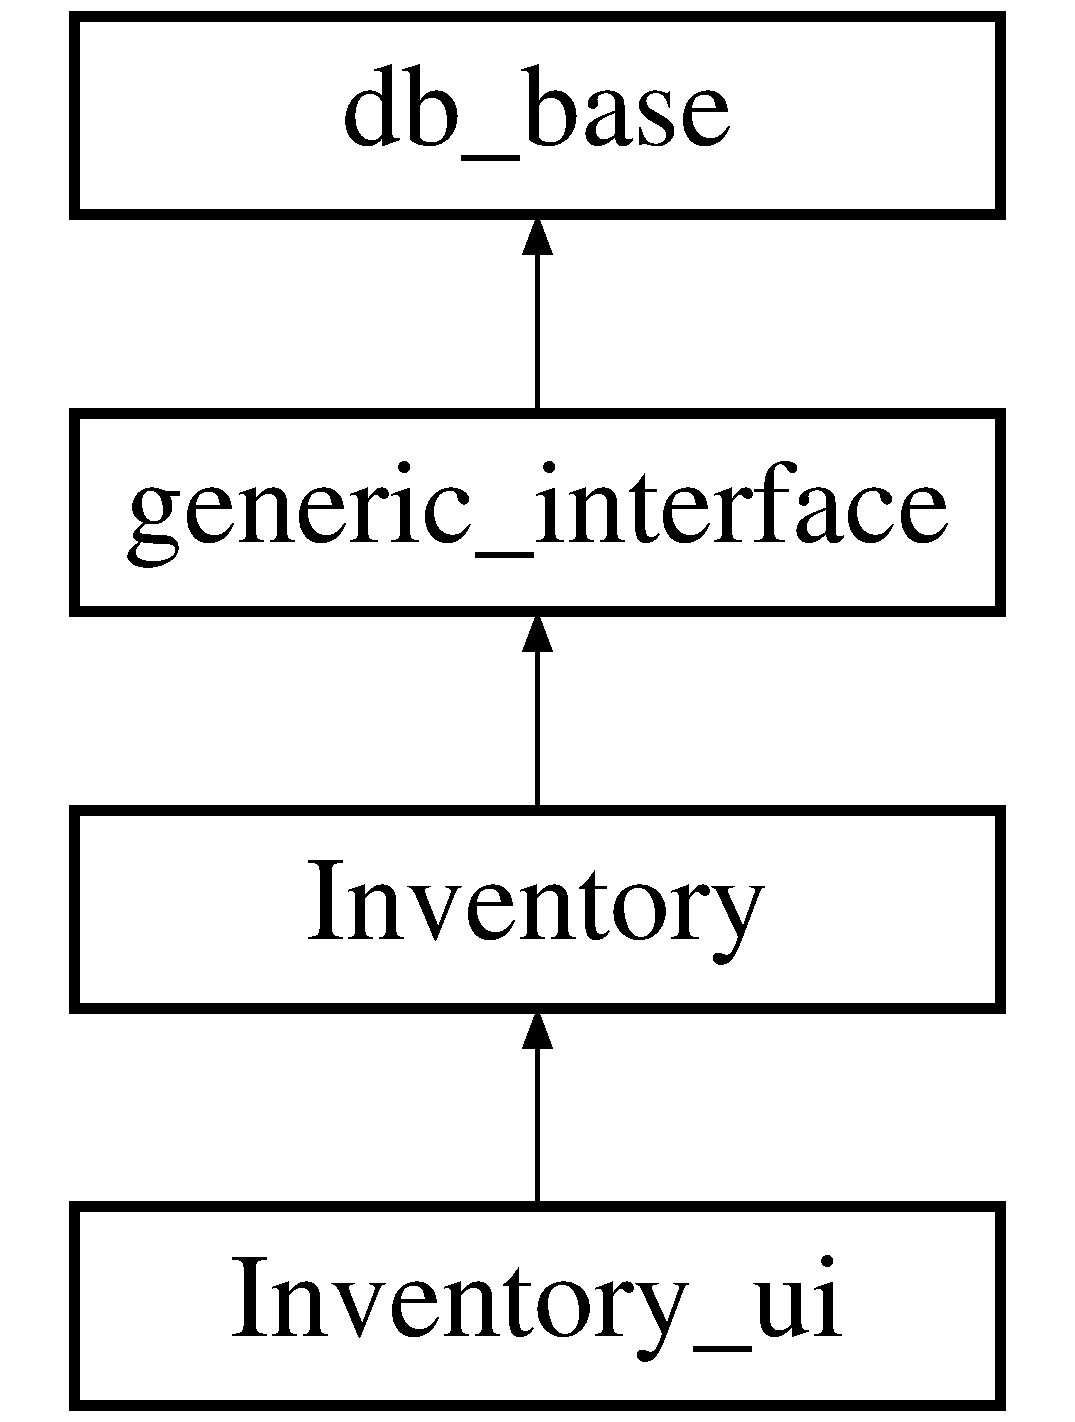
\includegraphics[height=4.000000cm]{dc/d4e/classgeneric__interface}
\end{center}
\end{figure}
\subsection*{Public Member Functions}
\begin{DoxyCompactItemize}
\item 
\hypertarget{classgeneric__interface_a1776ffb8e07b10eebcc6b71c7a057ea9}{}\label{classgeneric__interface_a1776ffb8e07b10eebcc6b71c7a057ea9} 
{\bfseries \+\_\+\+\_\+construct} (\$host, \$user, \$pass, \$database, \$prefs\+\_\+tablename)
\item 
\hypertarget{classgeneric__interface_af90523f08023ce9450f373f5c9dbf10e}{}\label{classgeneric__interface_af90523f08023ce9450f373f5c9dbf10e} 
{\bfseries related\+\_\+tabs} ()
\item 
\hypertarget{classgeneric__interface_a56cb641385fbc70dbb4496fcc87e6487}{}\label{classgeneric__interface_a56cb641385fbc70dbb4496fcc87e6487} 
{\bfseries show\+\_\+form} ()
\item 
\hypertarget{classgeneric__interface_ae447e539a3b57457ab7053131114dc72}{}\label{classgeneric__interface_ae447e539a3b57457ab7053131114dc72} 
{\bfseries base\+\_\+page} ()
\item 
\hypertarget{classgeneric__interface_afee00299dfab91da297364712a556128}{}\label{classgeneric__interface_afee00299dfab91da297364712a556128} 
{\bfseries display} ()
\item 
\hypertarget{classgeneric__interface_a2eda996cce2eb81ba95b3c13499f2a29}{}\label{classgeneric__interface_a2eda996cce2eb81ba95b3c13499f2a29} 
{\bfseries run} ()
\item 
\hypertarget{classgeneric__interface_ab12f6446b4f5986859cf5c3596d66e2f}{}\label{classgeneric__interface_ab12f6446b4f5986859cf5c3596d66e2f} 
{\bfseries append\+\_\+file} ( \$filename)
\item 
\hypertarget{classgeneric__interface_afa46d3c4fda07165bbf46c5b43177f01}{}\label{classgeneric__interface_afa46d3c4fda07165bbf46c5b43177f01} 
{\bfseries overwrite\+\_\+file} ( \$filename)
\item 
\hypertarget{classgeneric__interface_a2816e5f9355bb2051a08b36f5fe37b90}{}\label{classgeneric__interface_a2816e5f9355bb2051a08b36f5fe37b90} 
{\bfseries close\+\_\+file} ( \$fp)
\end{DoxyCompactItemize}
\subsection*{Public Attributes}
\begin{DoxyCompactItemize}
\item 
\hypertarget{classgeneric__interface_a0fed4a23a18ce292a0d7934b809c615d}{}\label{classgeneric__interface_a0fed4a23a18ce292a0d7934b809c615d} 
{\bfseries \$errors}
\item 
\hypertarget{classgeneric__interface_a69d365bc7157d8d74366b900ce99f584}{}\label{classgeneric__interface_a69d365bc7157d8d74366b900ce99f584} 
{\bfseries \$javascript}
\item 
\hypertarget{classgeneric__interface_a0ab93db3295a794300dac66c6e48bbb7}{}\label{classgeneric__interface_a0ab93db3295a794300dac66c6e48bbb7} 
{\bfseries \$help\+\_\+context}
\item 
\hypertarget{classgeneric__interface_a3537970983f08f4fabef6acfc21762d5}{}\label{classgeneric__interface_a3537970983f08f4fabef6acfc21762d5} 
{\bfseries \$page\+\_\+title}
\end{DoxyCompactItemize}


The documentation for this class was generated from the following file\+:\begin{DoxyCompactItemize}
\item 
class.\+generic\+\_\+interface.\+php\end{DoxyCompactItemize}

\hypertarget{classgeneric__orders}{}\section{generic\+\_\+orders Class Reference}
\label{classgeneric__orders}\index{generic\+\_\+orders@{generic\+\_\+orders}}
Inheritance diagram for generic\+\_\+orders\+:\begin{figure}[H]
\begin{center}
\leavevmode
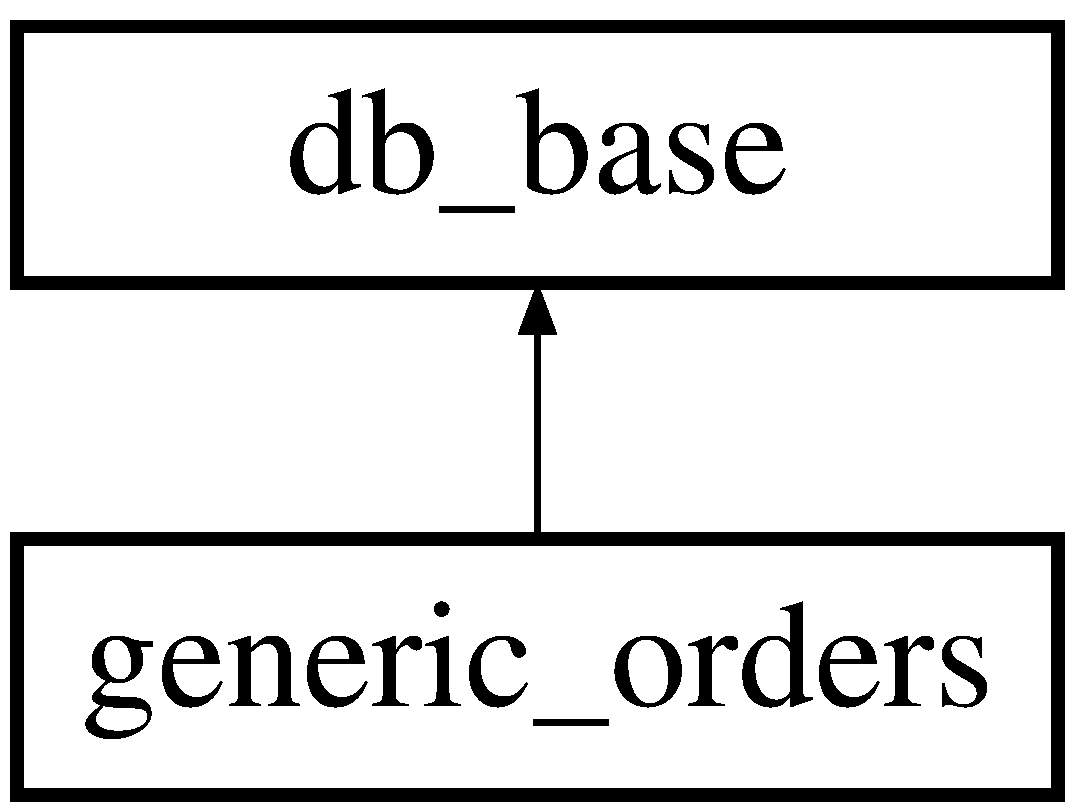
\includegraphics[height=2.000000cm]{d3/d2b/classgeneric__orders}
\end{center}
\end{figure}
\subsection*{Public Member Functions}
\begin{DoxyCompactItemize}
\item 
\hypertarget{classgeneric__orders_ad96a6adbcf3f1d2eaec7b3eefcf8cb8c}{}\label{classgeneric__orders_ad96a6adbcf3f1d2eaec7b3eefcf8cb8c} 
{\bfseries \+\_\+\+\_\+construct} ( \$host, \$user, \$pass, \$database, \$pref\+\_\+tablename)
\item 
\hypertarget{classgeneric__orders_a73da33c51344d619ad219c5c3533157a}{}\label{classgeneric__orders_a73da33c51344d619ad219c5c3533157a} 
{\bfseries install} ()
\item 
\hypertarget{classgeneric__orders_ac0a1f57dd5fe0ee9cad423a8581323b9}{}\label{classgeneric__orders_ac0a1f57dd5fe0ee9cad423a8581323b9} 
{\bfseries get\+\_\+purchase\+\_\+order} ()
\item 
\hypertarget{classgeneric__orders_a636930f29dd1a4214d9beb7b0b992fb2}{}\label{classgeneric__orders_a636930f29dd1a4214d9beb7b0b992fb2} 
{\bfseries get\+\_\+id\+\_\+range} ()
\item 
\hypertarget{classgeneric__orders_a77d76b233e40d4c76e7d93c4a2b87815}{}\label{classgeneric__orders_a77d76b233e40d4c76e7d93c4a2b87815} 
{\bfseries get\+\_\+supplier\+\_\+order} ()
\item 
\hypertarget{classgeneric__orders_afb2ea2f9acc44492b9f1880f31131df5}{}\label{classgeneric__orders_afb2ea2f9acc44492b9f1880f31131df5} 
{\bfseries export\+\_\+orders} ()
\item 
\hypertarget{classgeneric__orders_a5921f90917717297983148c16bfcdff7}{}\label{classgeneric__orders_a5921f90917717297983148c16bfcdff7} 
{\bfseries loadprefs} ()
\item 
\hypertarget{classgeneric__orders_a713ac2d657b69a5b68bcd93c085f6bff}{}\label{classgeneric__orders_a713ac2d657b69a5b68bcd93c085f6bff} 
{\bfseries updateprefs} ()
\item 
\hypertarget{classgeneric__orders_a733f9e1d53da1f2002ad5580d6215baf}{}\label{classgeneric__orders_a733f9e1d53da1f2002ad5580d6215baf} 
{\bfseries checkprefs} ()
\item 
\hypertarget{classgeneric__orders_a58246a65d39b0a1f79a520c54bf160a5}{}\label{classgeneric__orders_a58246a65d39b0a1f79a520c54bf160a5} 
{\bfseries action\+\_\+show\+\_\+form} ()
\item 
\hypertarget{classgeneric__orders_ae17ab2370a928c300c4900d1b14976d2}{}\label{classgeneric__orders_ae17ab2370a928c300c4900d1b14976d2} 
{\bfseries form\+\_\+export} ()
\item 
\hypertarget{classgeneric__orders_a9510fade9bbc4e505930f08750ef1c5f}{}\label{classgeneric__orders_a9510fade9bbc4e505930f08750ef1c5f} 
{\bfseries related\+\_\+tabs} ()
\item 
\hypertarget{classgeneric__orders_a04c2ba96918f5aed83649677feec28d5}{}\label{classgeneric__orders_a04c2ba96918f5aed83649677feec28d5} 
{\bfseries show\+\_\+form} ()
\item 
\hypertarget{classgeneric__orders_adda352a9a97d7d94b34e2ad5289643d2}{}\label{classgeneric__orders_adda352a9a97d7d94b34e2ad5289643d2} 
{\bfseries base\+\_\+page} ()
\item 
\hypertarget{classgeneric__orders_a30d91bc07b565db854032cf4687583b6}{}\label{classgeneric__orders_a30d91bc07b565db854032cf4687583b6} 
{\bfseries display} ()
\item 
\hypertarget{classgeneric__orders_aa26ae7d2601973a71a16a0f40a9946f8}{}\label{classgeneric__orders_aa26ae7d2601973a71a16a0f40a9946f8} 
{\bfseries run} ()
\end{DoxyCompactItemize}
\subsection*{Public Attributes}
\begin{DoxyCompactItemize}
\item 
\hypertarget{classgeneric__orders_a9a99b3d242d00f9dff29c452930cdc46}{}\label{classgeneric__orders_a9a99b3d242d00f9dff29c452930cdc46} 
{\bfseries \$order\+\_\+no}
\item 
\hypertarget{classgeneric__orders_a5b9ac946cce6674e2b7abcfd396f82ea}{}\label{classgeneric__orders_a5b9ac946cce6674e2b7abcfd396f82ea} 
{\bfseries \$db\+\_\+\+Host}
\item 
\hypertarget{classgeneric__orders_a24279845da685a00cf035df4bbe339d1}{}\label{classgeneric__orders_a24279845da685a00cf035df4bbe339d1} 
{\bfseries \$db\+\_\+\+User}
\item 
\hypertarget{classgeneric__orders_af6abeff7193a46c1785edef999aebe72}{}\label{classgeneric__orders_af6abeff7193a46c1785edef999aebe72} 
{\bfseries \$db\+\_\+\+Password}
\item 
\hypertarget{classgeneric__orders_ab37c01fb6bfad57f908e01b6c65e5d9d}{}\label{classgeneric__orders_ab37c01fb6bfad57f908e01b6c65e5d9d} 
{\bfseries \$db\+\_\+\+Name}
\item 
\hypertarget{classgeneric__orders_a723c673ed302846be920efe7ef6b656e}{}\label{classgeneric__orders_a723c673ed302846be920efe7ef6b656e} 
{\bfseries \$last\+\_\+order\+\_\+no}
\item 
\hypertarget{classgeneric__orders_a9eb2c59dd61c0dde32ff3171a522bd69}{}\label{classgeneric__orders_a9eb2c59dd61c0dde32ff3171a522bd69} 
{\bfseries \$vendor}
\item 
\hypertarget{classgeneric__orders_ae9ac8a364ccd57159c7c2f7cb9828444}{}\label{classgeneric__orders_ae9ac8a364ccd57159c7c2f7cb9828444} 
{\bfseries \$tabs} = array()
\item 
\hypertarget{classgeneric__orders_a8b5bbce48d66545ab58b43f4be772872}{}\label{classgeneric__orders_a8b5bbce48d66545ab58b43f4be772872} 
{\bfseries \$found}
\item 
\hypertarget{classgeneric__orders_ad9f0450540b7abed0a3952217421268b}{}\label{classgeneric__orders_ad9f0450540b7abed0a3952217421268b} 
{\bfseries \$purchase\+\_\+order}
\item 
\hypertarget{classgeneric__orders_aa9882dc26f8860b93d947905dfca7483}{}\label{classgeneric__orders_aa9882dc26f8860b93d947905dfca7483} 
{\bfseries \$config\+\_\+values} = array()
\item 
\hypertarget{classgeneric__orders_a0886ded57343072f2ad3821288d00454}{}\label{classgeneric__orders_a0886ded57343072f2ad3821288d00454} 
{\bfseries \$help\+\_\+context}
\item 
\hypertarget{classgeneric__orders_acfdc001bf2e21ac8d63d8265f3b2dd3f}{}\label{classgeneric__orders_acfdc001bf2e21ac8d63d8265f3b2dd3f} 
{\bfseries \$action}
\item 
\hypertarget{classgeneric__orders_ad884a4bee50042666a9c9aebece716bd}{}\label{classgeneric__orders_ad884a4bee50042666a9c9aebece716bd} 
{\bfseries \$redirect\+\_\+to}
\end{DoxyCompactItemize}


The documentation for this class was generated from the following file\+:\begin{DoxyCompactItemize}
\item 
class.\+generic\+\_\+orders.\+php\end{DoxyCompactItemize}

\hypertarget{classhooks___inventory}{}\section{hooks\+\_\+\+Inventory Class Reference}
\label{classhooks___inventory}\index{hooks\+\_\+\+Inventory@{hooks\+\_\+\+Inventory}}
Inheritance diagram for hooks\+\_\+\+Inventory\+:\begin{figure}[H]
\begin{center}
\leavevmode
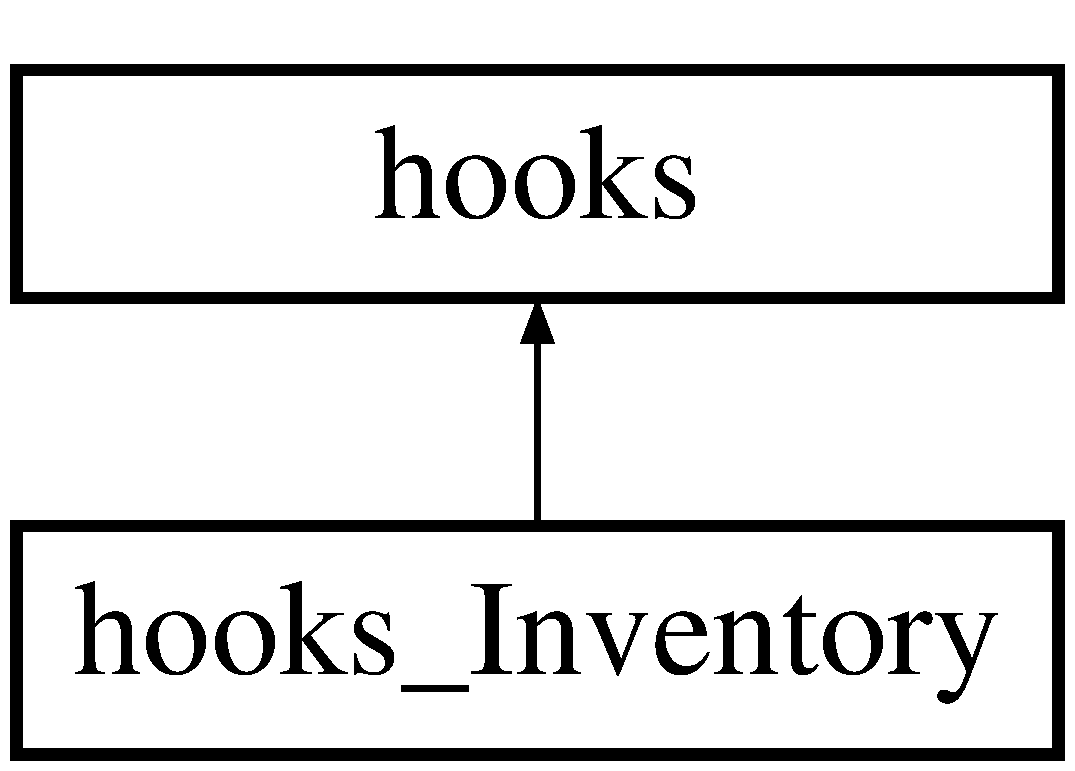
\includegraphics[height=2.000000cm]{dd/d41/classhooks___inventory}
\end{center}
\end{figure}
\subsection*{Public Member Functions}
\begin{DoxyCompactItemize}
\item 
\hyperlink{classhooks___inventory_a92994ac980fa7a6e8256e12c999cde84}{install\+\_\+options} (\$app)
\item 
\hyperlink{classhooks___inventory_ab5c9c0ba2bcb53683571ff27ab5000dd}{install\+\_\+access} ()
\end{DoxyCompactItemize}
\subsection*{Public Attributes}
\begin{DoxyCompactItemize}
\item 
\hypertarget{classhooks___inventory_a85ac46d599d8926eb60fd90b828dbccd}{}\label{classhooks___inventory_a85ac46d599d8926eb60fd90b828dbccd} 
\hyperlink{classhooks___inventory_a85ac46d599d8926eb60fd90b828dbccd}{\$module\+\_\+name} = \textquotesingle{}\hyperlink{class_inventory}{Inventory}\textquotesingle{}
\begin{DoxyCompactList}\small\item\em Module Name so that I only have to replace in one place for easier copy and paste to new modules. \end{DoxyCompactList}\end{DoxyCompactItemize}


\subsection{Detailed Description}
class \hyperlink{classhooks___inventory}{hooks\+\_\+\+Inventory} extends hooks as required by the Front\+Accounting A\+PI. 

\subsection{Member Function Documentation}
\hypertarget{classhooks___inventory_ab5c9c0ba2bcb53683571ff27ab5000dd}{}\label{classhooks___inventory_ab5c9c0ba2bcb53683571ff27ab5000dd} 
\index{hooks\+\_\+\+Inventory@{hooks\+\_\+\+Inventory}!install\+\_\+access@{install\+\_\+access}}
\index{install\+\_\+access@{install\+\_\+access}!hooks\+\_\+\+Inventory@{hooks\+\_\+\+Inventory}}
\subsubsection{\texorpdfstring{install\+\_\+access()}{install\_access()}}
{\footnotesize\ttfamily hooks\+\_\+\+Inventory\+::install\+\_\+access (\begin{DoxyParamCaption}{ }\end{DoxyParamCaption})}

Install\+\_\+access sets up the Security settings for FA 
\begin{DoxyParams}{Parameters}
{\em none} & \\
\hline
\end{DoxyParams}
\begin{DoxyReturn}{Returns}
array 
\end{DoxyReturn}
\hypertarget{classhooks___inventory_a92994ac980fa7a6e8256e12c999cde84}{}\label{classhooks___inventory_a92994ac980fa7a6e8256e12c999cde84} 
\index{hooks\+\_\+\+Inventory@{hooks\+\_\+\+Inventory}!install\+\_\+options@{install\+\_\+options}}
\index{install\+\_\+options@{install\+\_\+options}!hooks\+\_\+\+Inventory@{hooks\+\_\+\+Inventory}}
\subsubsection{\texorpdfstring{install\+\_\+options()}{install\_options()}}
{\footnotesize\ttfamily hooks\+\_\+\+Inventory\+::install\+\_\+options (\begin{DoxyParamCaption}\item[{}]{\$app }\end{DoxyParamCaption})}

Install additonal menu options provided by module 
\begin{DoxyParams}{Parameters}
{\em app} & object \\
\hline
\end{DoxyParams}
\begin{DoxyReturn}{Returns}
nothing 
\end{DoxyReturn}


The documentation for this class was generated from the following file\+:\begin{DoxyCompactItemize}
\item 
hooks.\+php\end{DoxyCompactItemize}

\hypertarget{class_inventory}{}\section{Inventory Class Reference}
\label{class_inventory}\index{Inventory@{Inventory}}
Inheritance diagram for Inventory\+:\begin{figure}[H]
\begin{center}
\leavevmode
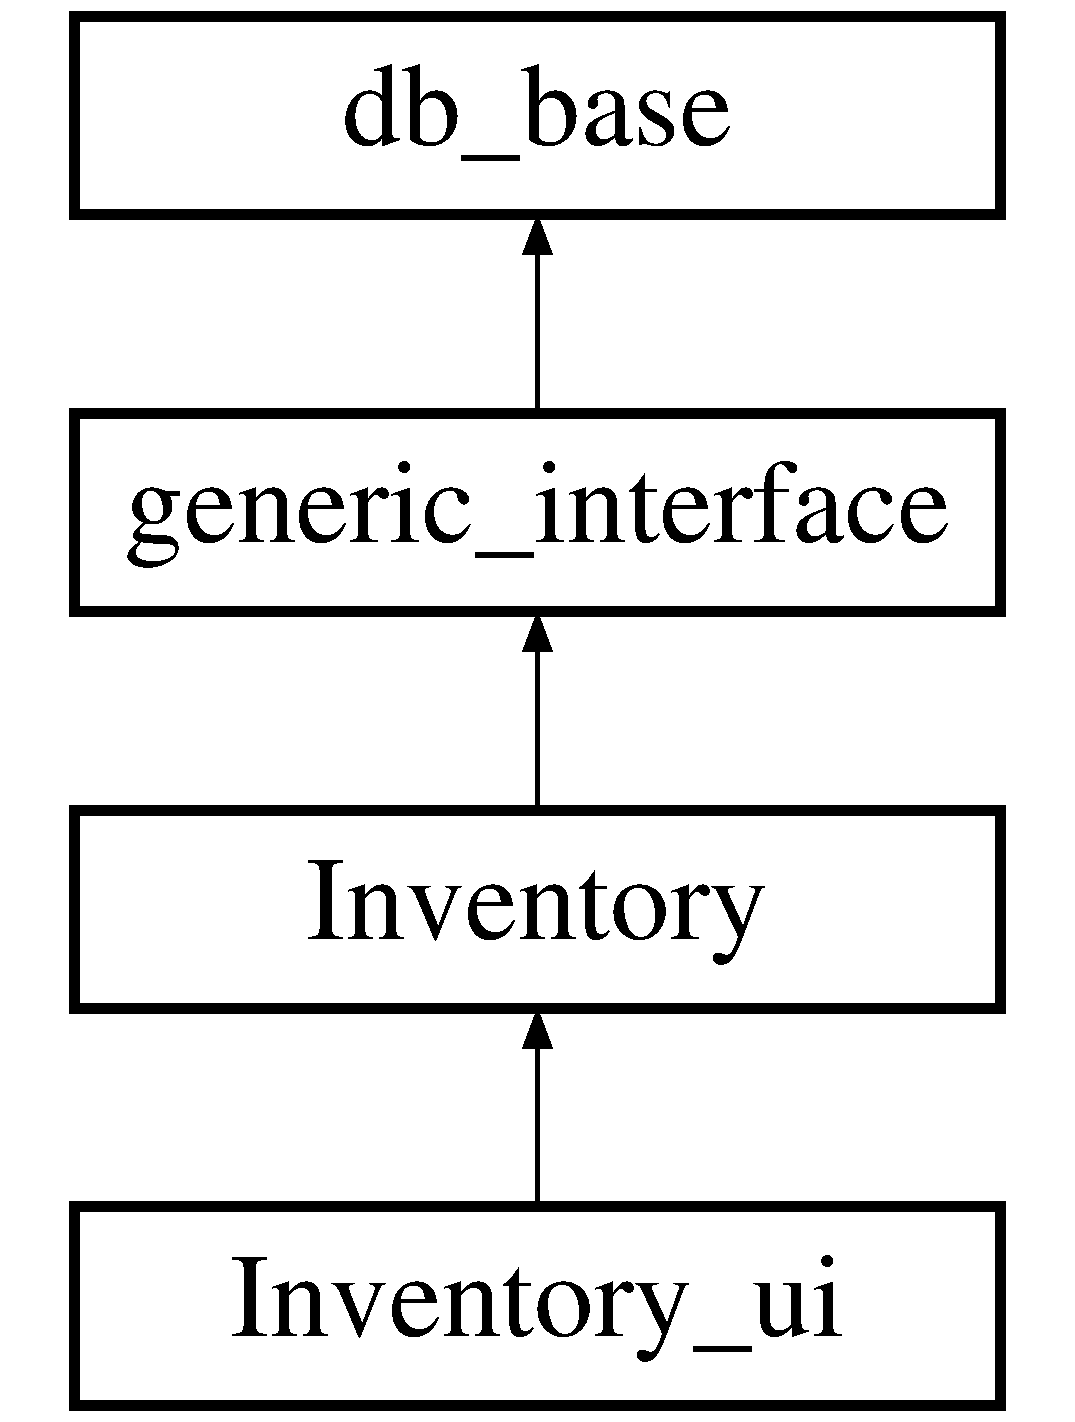
\includegraphics[height=4.000000cm]{da/d71/class_inventory}
\end{center}
\end{figure}
\subsection*{Public Member Functions}
\begin{DoxyCompactItemize}
\item 
\hyperlink{class_inventory_a3d94ae6f942f9c10ba12a75b57ec1d43}{\+\_\+\+\_\+construct} ( \$host, \$user, \$pass, \$database, \$pref\+\_\+tablename)
\item 
\hypertarget{class_inventory_a8e1cc8e71fe7c1340e246f23a9c14b7a}{}\label{class_inventory_a8e1cc8e71fe7c1340e246f23a9c14b7a} 
{\bfseries install} ()
\item 
\hypertarget{class_inventory_aabb97aaa0e58e324b6077cc0a5593384}{}\label{class_inventory_aabb97aaa0e58e324b6077cc0a5593384} 
{\bfseries write} ()
\item 
\hypertarget{class_inventory_a1c90cc40b9139610f3db802b67d7c211}{}\label{class_inventory_a1c90cc40b9139610f3db802b67d7c211} 
{\bfseries process\+\_\+inventory} ()
\item 
\hyperlink{class_inventory_a47208c8f736cae33d5293f0c160266cb}{copy\+\_\+from\+\_\+session} ()
\item 
\hypertarget{class_inventory_a5d05f6203e1f1d0d26b4ad1a6ee416b0}{}\label{class_inventory_a5d05f6203e1f1d0d26b4ad1a6ee416b0} 
{\bfseries copy\+\_\+to\+\_\+session} ()
\item 
\hyperlink{class_inventory_a05cfd3bab20f8d1d40a8f83beb23d694}{can\+\_\+process} ()
\item 
\hypertarget{class_inventory_afe4428608c97c76ee1e5f7bbd6ce4083}{}\label{class_inventory_afe4428608c97c76ee1e5f7bbd6ce4083} 
{\bfseries handle\+\_\+update\+\_\+item} ()
\item 
\hypertarget{class_inventory_a9460265e3641d0fa9f14fe584d2369c0}{}\label{class_inventory_a9460265e3641d0fa9f14fe584d2369c0} 
{\bfseries delete\+\_\+all\+\_\+items} ()
\item 
\hypertarget{class_inventory_a509402207c6adb506bbd9a22a15415e9}{}\label{class_inventory_a509402207c6adb506bbd9a22a15415e9} 
{\bfseries handle\+\_\+delete\+\_\+item} (\$line\+\_\+no)
\item 
\hypertarget{class_inventory_ac66fe979ed1b2d30e64972356757df8c}{}\label{class_inventory_ac66fe979ed1b2d30e64972356757df8c} 
{\bfseries is\+Stockid} ( \$stock\+\_\+id)
\item 
\hyperlink{class_inventory_ac788e157a403fd8192b4dd2eedf57378}{is\+Item\+Code} ( \$item\+\_\+code)
\item 
\hypertarget{class_inventory_a56d65f3277dff3761e841f2c0a7909d2}{}\label{class_inventory_a56d65f3277dff3761e841f2c0a7909d2} 
{\bfseries get\+\_\+item\+\_\+description} ()
\item 
\hypertarget{class_inventory_ad141ddfa4b1b812f60ef7ad0ef8d391f}{}\label{class_inventory_ad141ddfa4b1b812f60ef7ad0ef8d391f} 
{\bfseries add\+\_\+item} ()
\item 
\hyperlink{class_inventory_a20a38a02a619c23ac051bef0f804b533}{find\+\_\+cart\+\_\+item} ()
\item 
\hypertarget{class_inventory_a4bd02c483dcc9f4f76ccb86a4aee44f4}{}\label{class_inventory_a4bd02c483dcc9f4f76ccb86a4aee44f4} 
{\bfseries handle\+\_\+new\+\_\+item} ()
\item 
\hyperlink{class_inventory_a2ff0a0bf19271240f31d948ac2373141}{clearcart} ()
\item 
\hyperlink{class_inventory_a6fb9d26bbc7d5385e77dd2fd01da307b}{create\+\_\+cart} ()
\item 
\hyperlink{class_inventory_a5a32d543b372a64b4def7948d4582c9b}{has\+Barcode} ()
\item 
\hyperlink{class_inventory_ab93ab1de4e3622b63b07a3ec17bb5753}{get\+\_\+item\+\_\+qoh\+\_\+location} ( \$stock\+\_\+id)
\item 
\hyperlink{class_inventory_abe1f31716dc97f457dc66411526cfcc6}{get\+\_\+items\+\_\+qoh\+\_\+location} ()
\item 
\hyperlink{class_inventory_abcdb59c12133ade607ed4ef6d80bec94}{call\+\_\+table} ( \$action, \$msg)
\item 
\hypertarget{class_inventory_a5980667d55e7f4df41ee1ca8c6e4e1f7}{}\label{class_inventory_a5980667d55e7f4df41ee1ca8c6e4e1f7} 
{\bfseries xfer\+\_\+all\+\_\+settings} ( \$action)
\item 
\hypertarget{class_inventory_a9f10a2dacd1fa4e3b82c7d62f451bb4b}{}\label{class_inventory_a9f10a2dacd1fa4e3b82c7d62f451bb4b} 
{\bfseries add\+\_\+all\+\_\+list} ( \$action=\char`\"{}zero\char`\"{})
\item 
\hypertarget{class_inventory_aa794599f6f24788a4eea4343ecd90cdb}{}\label{class_inventory_aa794599f6f24788a4eea4343ecd90cdb} 
{\bfseries handle\+\_\+new\+\_\+inventory} ()
\item 
\hypertarget{class_inventory_a27f4d6058f0ed5decaaabbec1408f39e}{}\label{class_inventory_a27f4d6058f0ed5decaaabbec1408f39e} 
{\bfseries init\+\_\+tables\+\_\+completed} ()
\item 
\hypertarget{class_inventory_af8d9a21653be97fe48c954893313733b}{}\label{class_inventory_af8d9a21653be97fe48c954893313733b} 
{\bfseries create\+\_\+table\+\_\+inventory\+\_\+last\+\_\+performed} ()
\item 
\hypertarget{class_inventory_abac339a921acc7633bad02779bff228b}{}\label{class_inventory_abac339a921acc7633bad02779bff228b} 
{\bfseries record\+\_\+last\+\_\+inv\+\_\+date} ( \$stock\+\_\+id)
\item 
\hypertarget{class_inventory_abbef2528107ec0d7d4bb1a0c4dd2ada4}{}\label{class_inventory_abbef2528107ec0d7d4bb1a0c4dd2ada4} 
{\bfseries process} ()
\end{DoxyCompactItemize}
\subsection*{Public Attributes}
\begin{DoxyCompactItemize}
\item 
\hypertarget{class_inventory_aa787e03e29020e679e25b6504711f908}{}\label{class_inventory_aa787e03e29020e679e25b6504711f908} 
{\bfseries \$location}
\item 
\hypertarget{class_inventory_aecb8d5b7cc910234b879b6d014e887ed}{}\label{class_inventory_aecb8d5b7cc910234b879b6d014e887ed} 
\hyperlink{class_inventory_aecb8d5b7cc910234b879b6d014e887ed}{\$holdtank}
\begin{DoxyCompactList}\small\item\em Location that acts as holding tank for corrections. Config Value. \end{DoxyCompactList}\item 
\hypertarget{class_inventory_ae8dc058519cb65b6f98c5b861e9b4b6c}{}\label{class_inventory_ae8dc058519cb65b6f98c5b861e9b4b6c} 
\hyperlink{class_inventory_ae8dc058519cb65b6f98c5b861e9b4b6c}{\$to\+\_\+location}
\begin{DoxyCompactList}\small\item\em Used for the xfer\+\_\+all functions. \end{DoxyCompactList}\item 
\hypertarget{class_inventory_add61c6c29ac22e95ff7393f247b4cf24}{}\label{class_inventory_add61c6c29ac22e95ff7393f247b4cf24} 
\hyperlink{class_inventory_add61c6c29ac22e95ff7393f247b4cf24}{\$from\+\_\+location}
\begin{DoxyCompactList}\small\item\em Used for the xfer\+\_\+all functions. \end{DoxyCompactList}\item 
\hypertarget{class_inventory_a23522a816fa22f04ddbe1bb7fe55db56}{}\label{class_inventory_a23522a816fa22f04ddbe1bb7fe55db56} 
{\bfseries \$url}
\item 
\hypertarget{class_inventory_a09b60b4e48ba34b348a644aad86bc914}{}\label{class_inventory_a09b60b4e48ba34b348a644aad86bc914} 
{\bfseries \$trans\+\_\+type}
\item 
\hypertarget{class_inventory_a6c461cfddac57ddd5f56f394cee33328}{}\label{class_inventory_a6c461cfddac57ddd5f56f394cee33328} 
{\bfseries \$trans\+\_\+no}
\item 
\hypertarget{class_inventory_a4b9f25d8866f4f876d1646b1a5f693df}{}\label{class_inventory_a4b9f25d8866f4f876d1646b1a5f693df} 
{\bfseries \$barcode}
\item 
\hypertarget{class_inventory_a111643a727ee9481ab774c5a2ca40ee8}{}\label{class_inventory_a111643a727ee9481ab774c5a2ca40ee8} 
{\bfseries \$location\+Prefix}
\item 
\hypertarget{class_inventory_a636172fcf4605cce00cefe5b753acb44}{}\label{class_inventory_a636172fcf4605cce00cefe5b753acb44} 
{\bfseries \$location\+Prefix2}
\item 
\hypertarget{class_inventory_aefba336f82cf7c89b2ab89c4f732d9c5}{}\label{class_inventory_aefba336f82cf7c89b2ab89c4f732d9c5} 
{\bfseries \$line\+\_\+items}
\item 
\hypertarget{class_inventory_a62106a6a3b9f340a4493d0e638a9fb21}{}\label{class_inventory_a62106a6a3b9f340a4493d0e638a9fb21} 
{\bfseries \$reference}
\item 
\hypertarget{class_inventory_a47686bff60ceb7967af2b8c5395bc40e}{}\label{class_inventory_a47686bff60ceb7967af2b8c5395bc40e} 
{\bfseries \$\+Comments}
\item 
\hypertarget{class_inventory_a151f90398aa3afc94c3ab5eef340943b}{}\label{class_inventory_a151f90398aa3afc94c3ab5eef340943b} 
{\bfseries \$document\+\_\+date}
\item 
\hypertarget{class_inventory_add9d7263f9803f41cc37cb3d57a9f28c}{}\label{class_inventory_add9d7263f9803f41cc37cb3d57a9f28c} 
{\bfseries \$ex\+\_\+rate}
\item 
\hypertarget{class_inventory_a43ce64bb2165484553d6c95406764e4c}{}\label{class_inventory_a43ce64bb2165484553d6c95406764e4c} 
{\bfseries \$deliver\+\_\+to}
\item 
\hypertarget{class_inventory_a017f82d9a4aa2f57753cbd473a7be595}{}\label{class_inventory_a017f82d9a4aa2f57753cbd473a7be595} 
{\bfseries \$delivery\+\_\+address}
\item 
\hypertarget{class_inventory_a6e30b011ebf9c05093679577559aceeb}{}\label{class_inventory_a6e30b011ebf9c05093679577559aceeb} 
{\bfseries \$copyfromcount}
\item 
\hypertarget{class_inventory_a4235854bd547f566b916bc56c479a644}{}\label{class_inventory_a4235854bd547f566b916bc56c479a644} 
{\bfseries \$copytocount}
\item 
\hypertarget{class_inventory_a85828227481d0b6af837a2924bc69c2e}{}\label{class_inventory_a85828227481d0b6af837a2924bc69c2e} 
{\bfseries \$title}
\item 
\hypertarget{class_inventory_ad41a55d723a128faa987dd710a1d7d14}{}\label{class_inventory_ad41a55d723a128faa987dd710a1d7d14} 
{\bfseries \$path\+\_\+to\+\_\+root}
\item 
\hypertarget{class_inventory_a22a5cb92bfa2d65eb7070e8c5164ba61}{}\label{class_inventory_a22a5cb92bfa2d65eb7070e8c5164ba61} 
{\bfseries \$update\+\_\+quantity}
\item 
\hypertarget{class_inventory_a0cade591b02c5dc6e280d7d90e2fa3b4}{}\label{class_inventory_a0cade591b02c5dc6e280d7d90e2fa3b4} 
{\bfseries \$add\+\_\+quantity}
\item 
\hypertarget{class_inventory_aff1f3648941f2cd2c8e787989b679bb8}{}\label{class_inventory_aff1f3648941f2cd2c8e787989b679bb8} 
{\bfseries \$item\+\_\+text}
\item 
\hypertarget{class_inventory_ac6b30b7db054bca3509a961d4b21143d}{}\label{class_inventory_ac6b30b7db054bca3509a961d4b21143d} 
{\bfseries \$stock\+\_\+id}
\item 
\hypertarget{class_inventory_ae2d8bc329f9ebbdfd75325b5e8f27a59}{}\label{class_inventory_ae2d8bc329f9ebbdfd75325b5e8f27a59} 
{\bfseries \$change\+\_\+line\+\_\+number}
\item 
\hypertarget{class_inventory_a886ee1cbe6cb6a36a4573057f41bef25}{}\label{class_inventory_a886ee1cbe6cb6a36a4573057f41bef25} 
{\bfseries \$table\+\_\+interface}
\end{DoxyCompactItemize}


\subsection{Detailed Description}
Class \hyperlink{class_inventory}{Inventory} is the routines for doing a stock taking.

Class \hyperlink{class_inventory}{Inventory} is the routines for doing a stock taking. It also allows you to do inventory transfers of A\+LL inventory without having to count those items at both locations. A\+S\+S\+U\+M\+P\+T\+I\+ON is that you will do an appropriate inventory count later. 

\subsection{Constructor \& Destructor Documentation}
\hypertarget{class_inventory_a3d94ae6f942f9c10ba12a75b57ec1d43}{}\label{class_inventory_a3d94ae6f942f9c10ba12a75b57ec1d43} 
\index{Inventory@{Inventory}!\+\_\+\+\_\+construct@{\+\_\+\+\_\+construct}}
\index{\+\_\+\+\_\+construct@{\+\_\+\+\_\+construct}!Inventory@{Inventory}}
\subsubsection{\texorpdfstring{\+\_\+\+\_\+construct()}{\_\_construct()}}
{\footnotesize\ttfamily Inventory\+::\+\_\+\+\_\+construct (\begin{DoxyParamCaption}\item[{}]{\$host,  }\item[{}]{\$user,  }\item[{}]{\$pass,  }\item[{}]{\$database,  }\item[{}]{\$pref\+\_\+tablename }\end{DoxyParamCaption})}

Constructor

The params for this constructor are not needed for this particular function; They are needed for compatibility to \hyperlink{classgeneric__interface}{generic\+\_\+interface} which this class extends so that we don\textquotesingle{}t break the parent constructor.

Generic\+\_\+interface gives us the routines that allow us to set actions and the forms/routines that we are supposed to then call without having to write a bunch of if/then/else statements. (see \$this-\/$>$tabs). It also gives us the generic C\+O\+N\+F\+IG V\+A\+R\+I\+A\+B\+L\+ES (see \$this-\/$>$config\+\_\+values) which are then presented on the configuration tab, and stored in the modules prefs table. 

\subsection{Member Function Documentation}
\hypertarget{class_inventory_abcdb59c12133ade607ed4ef6d80bec94}{}\label{class_inventory_abcdb59c12133ade607ed4ef6d80bec94} 
\index{Inventory@{Inventory}!call\+\_\+table@{call\+\_\+table}}
\index{call\+\_\+table@{call\+\_\+table}!Inventory@{Inventory}}
\subsubsection{\texorpdfstring{call\+\_\+table()}{call\_table()}}
{\footnotesize\ttfamily Inventory\+::call\+\_\+table (\begin{DoxyParamCaption}\item[{}]{\$action,  }\item[{}]{\$msg }\end{DoxyParamCaption})}

Routine to display a table with a button so we can call an action function. Also in generic\+\_\+fa\+\_\+interface?


\begin{DoxyParams}{Parameters}
{\em string} & action \\
\hline
{\em string} & display on button \\
\hline
\end{DoxyParams}
\begin{DoxyReturn}{Returns}
null 
\end{DoxyReturn}
\hypertarget{class_inventory_a05cfd3bab20f8d1d40a8f83beb23d694}{}\label{class_inventory_a05cfd3bab20f8d1d40a8f83beb23d694} 
\index{Inventory@{Inventory}!can\+\_\+process@{can\+\_\+process}}
\index{can\+\_\+process@{can\+\_\+process}!Inventory@{Inventory}}
\subsubsection{\texorpdfstring{can\+\_\+process()}{can\_process()}}
{\footnotesize\ttfamily Inventory\+::can\+\_\+process (\begin{DoxyParamCaption}{ }\end{DoxyParamCaption})}

Can we process the data? \begin{DoxyWarning}{Warning}
requires reference, document\+\_\+date to be set, will set if not 

requires from\+\_\+location and to\+\_\+location to be set. 
\end{DoxyWarning}

\begin{DoxyExceptions}{Exceptions}
{\em Exception} & \\
\hline
\end{DoxyExceptions}
\begin{DoxyReturn}{Returns}
Bool yes or no 
\end{DoxyReturn}
\hypertarget{class_inventory_a2ff0a0bf19271240f31d948ac2373141}{}\label{class_inventory_a2ff0a0bf19271240f31d948ac2373141} 
\index{Inventory@{Inventory}!clearcart@{clearcart}}
\index{clearcart@{clearcart}!Inventory@{Inventory}}
\subsubsection{\texorpdfstring{clearcart()}{clearcart()}}
{\footnotesize\ttfamily Inventory\+::clearcart (\begin{DoxyParamCaption}{ }\end{DoxyParamCaption})}

Clear the list of items in the cart

none \begin{DoxyReturn}{Returns}
null 
\end{DoxyReturn}
\hypertarget{class_inventory_a47208c8f736cae33d5293f0c160266cb}{}\label{class_inventory_a47208c8f736cae33d5293f0c160266cb} 
\index{Inventory@{Inventory}!copy\+\_\+from\+\_\+session@{copy\+\_\+from\+\_\+session}}
\index{copy\+\_\+from\+\_\+session@{copy\+\_\+from\+\_\+session}!Inventory@{Inventory}}
\subsubsection{\texorpdfstring{copy\+\_\+from\+\_\+session()}{copy\_from\_session()}}
{\footnotesize\ttfamily Inventory\+::copy\+\_\+from\+\_\+session (\begin{DoxyParamCaption}{ }\end{DoxyParamCaption})}

copy\+\_\+from\+\_\+session Copies out of \$\+\_\+\+S\+E\+S\+S\+I\+ON into a C\+A\+RT structure the line items including stock\+\_\+id, qoh, quantity, etc. Also includes from\+\_\+location and to\+\_\+location


\begin{DoxyParams}{Parameters}
{\em N\+O\+NE} & \\
\hline
\end{DoxyParams}
\begin{DoxyReturn}{Returns}
N\+O\+NE 
\end{DoxyReturn}
\hypertarget{class_inventory_a6fb9d26bbc7d5385e77dd2fd01da307b}{}\label{class_inventory_a6fb9d26bbc7d5385e77dd2fd01da307b} 
\index{Inventory@{Inventory}!create\+\_\+cart@{create\+\_\+cart}}
\index{create\+\_\+cart@{create\+\_\+cart}!Inventory@{Inventory}}
\subsubsection{\texorpdfstring{create\+\_\+cart()}{create\_cart()}}
{\footnotesize\ttfamily Inventory\+::create\+\_\+cart (\begin{DoxyParamCaption}{ }\end{DoxyParamCaption})}

Create a new cart.

none \begin{DoxyReturn}{Returns}
null 
\end{DoxyReturn}
\hypertarget{class_inventory_a20a38a02a619c23ac051bef0f804b533}{}\label{class_inventory_a20a38a02a619c23ac051bef0f804b533} 
\index{Inventory@{Inventory}!find\+\_\+cart\+\_\+item@{find\+\_\+cart\+\_\+item}}
\index{find\+\_\+cart\+\_\+item@{find\+\_\+cart\+\_\+item}!Inventory@{Inventory}}
\subsubsection{\texorpdfstring{find\+\_\+cart\+\_\+item()}{find\_cart\_item()}}
{\footnotesize\ttfamily Inventory\+::find\+\_\+cart\+\_\+item (\begin{DoxyParamCaption}{ }\end{DoxyParamCaption})}

Goes through the cart and returns the 0-\/based index if the P\+O\+ST\mbox{[}\textquotesingle{}stock\+\_\+id\textquotesingle{}\mbox{]}/barcode in cart.

none \begin{DoxyReturn}{Returns}
int (-\/1 on not found) 
\end{DoxyReturn}
\hypertarget{class_inventory_ab93ab1de4e3622b63b07a3ec17bb5753}{}\label{class_inventory_ab93ab1de4e3622b63b07a3ec17bb5753} 
\index{Inventory@{Inventory}!get\+\_\+item\+\_\+qoh\+\_\+location@{get\+\_\+item\+\_\+qoh\+\_\+location}}
\index{get\+\_\+item\+\_\+qoh\+\_\+location@{get\+\_\+item\+\_\+qoh\+\_\+location}!Inventory@{Inventory}}
\subsubsection{\texorpdfstring{get\+\_\+item\+\_\+qoh\+\_\+location()}{get\_item\_qoh\_location()}}
{\footnotesize\ttfamily Inventory\+::get\+\_\+item\+\_\+qoh\+\_\+location (\begin{DoxyParamCaption}\item[{}]{\$stock\+\_\+id }\end{DoxyParamCaption})}

Gets the Quantity On Hand for an item at a location on a date.

string stock\+\_\+id \begin{DoxyReturn}{Returns}
int 
\end{DoxyReturn}
\hypertarget{class_inventory_abe1f31716dc97f457dc66411526cfcc6}{}\label{class_inventory_abe1f31716dc97f457dc66411526cfcc6} 
\index{Inventory@{Inventory}!get\+\_\+items\+\_\+qoh\+\_\+location@{get\+\_\+items\+\_\+qoh\+\_\+location}}
\index{get\+\_\+items\+\_\+qoh\+\_\+location@{get\+\_\+items\+\_\+qoh\+\_\+location}!Inventory@{Inventory}}
\subsubsection{\texorpdfstring{get\+\_\+items\+\_\+qoh\+\_\+location()}{get\_items\_qoh\_location()}}
{\footnotesize\ttfamily Inventory\+::get\+\_\+items\+\_\+qoh\+\_\+location (\begin{DoxyParamCaption}{ }\end{DoxyParamCaption})}

Gets the Quantity On Hand for all items in the cart for a location on a date.

none \begin{DoxyReturn}{Returns}
null 
\end{DoxyReturn}
\hypertarget{class_inventory_a5a32d543b372a64b4def7948d4582c9b}{}\label{class_inventory_a5a32d543b372a64b4def7948d4582c9b} 
\index{Inventory@{Inventory}!has\+Barcode@{has\+Barcode}}
\index{has\+Barcode@{has\+Barcode}!Inventory@{Inventory}}
\subsubsection{\texorpdfstring{has\+Barcode()}{hasBarcode()}}
{\footnotesize\ttfamily Inventory\+::has\+Barcode (\begin{DoxyParamCaption}{ }\end{DoxyParamCaption})}

Check to see if the class has barcode set to anything other than \char`\"{}\char`\"{}.

none \begin{DoxyReturn}{Returns}
bool 
\end{DoxyReturn}
\hypertarget{class_inventory_ac788e157a403fd8192b4dd2eedf57378}{}\label{class_inventory_ac788e157a403fd8192b4dd2eedf57378} 
\index{Inventory@{Inventory}!is\+Item\+Code@{is\+Item\+Code}}
\index{is\+Item\+Code@{is\+Item\+Code}!Inventory@{Inventory}}
\subsubsection{\texorpdfstring{is\+Item\+Code()}{isItemCode()}}
{\footnotesize\ttfamily Inventory\+::is\+Item\+Code (\begin{DoxyParamCaption}\item[{}]{\$item\+\_\+code }\end{DoxyParamCaption})}

Code is in item\+\_\+code table but isn\textquotesingle{}t the stock\+\_\+id


\begin{DoxyParams}{Parameters}
{\em string} & \\
\hline
\end{DoxyParams}
\begin{DoxyReturn}{Returns}
bool 
\end{DoxyReturn}


The documentation for this class was generated from the following file\+:\begin{DoxyCompactItemize}
\item 
class.\+Inventory.\+php\end{DoxyCompactItemize}

\hypertarget{classinventory__cart}{}\section{inventory\+\_\+cart Class Reference}
\label{classinventory__cart}\index{inventory\+\_\+cart@{inventory\+\_\+cart}}
\subsection*{Public Member Functions}
\begin{DoxyCompactItemize}
\item 
\hypertarget{classinventory__cart_ad181b1f15c4e0342cd9cd54df9a2c8b7}{}\label{classinventory__cart_ad181b1f15c4e0342cd9cd54df9a2c8b7} 
{\bfseries \+\_\+\+\_\+construct} ( \$date=null)
\item 
\hypertarget{classinventory__cart_aa609c5eeaf39f8fe416ac2093d81d94b}{}\label{classinventory__cart_aa609c5eeaf39f8fe416ac2093d81d94b} 
{\bfseries new\+\_\+item} ( \$stock\+\_\+id)
\item 
\hypertarget{classinventory__cart_a1d31465361c00aad624a82933b3c1d63}{}\label{classinventory__cart_a1d31465361c00aad624a82933b3c1d63} 
{\bfseries serialize} ()
\item 
\hypertarget{classinventory__cart_ac988218bdcff3a458f505c4999e3e4b3}{}\label{classinventory__cart_ac988218bdcff3a458f505c4999e3e4b3} 
{\bfseries unserialize} (\$data)
\item 
\hypertarget{classinventory__cart_a6ca9bac672c850544da5ec593d89458f}{}\label{classinventory__cart_a6ca9bac672c850544da5ec593d89458f} 
{\bfseries cart2session} ()
\item 
\hypertarget{classinventory__cart_a62b8732c8d7f083f58c7839d020c0ba6}{}\label{classinventory__cart_a62b8732c8d7f083f58c7839d020c0ba6} 
{\bfseries session2cart} ()
\item 
\hypertarget{classinventory__cart_aa47a62325020ad6b5eb6acf5927ce65a}{}\label{classinventory__cart_aa47a62325020ad6b5eb6acf5927ce65a} 
{\bfseries can\+\_\+process} ()
\item 
\hypertarget{classinventory__cart_a00e14d7734a32d9192631ab8349d024e}{}\label{classinventory__cart_a00e14d7734a32d9192631ab8349d024e} 
{\bfseries handle\+\_\+update\+\_\+item} ()
\item 
\hypertarget{classinventory__cart_ae283c95df0a280d6037ad59d0f6e71f1}{}\label{classinventory__cart_ae283c95df0a280d6037ad59d0f6e71f1} 
{\bfseries handle\+\_\+delete\+\_\+item} (\$line\+\_\+no)
\item 
\hyperlink{classinventory__cart_af2060bcea0c8fd54ae0a2e5550a44935}{increment\+\_\+item\+\_\+count} ( \$stock\+\_\+id, \$count)
\item 
\hypertarget{classinventory__cart_ada03f4b41aa7aef0b29aa187a09ae857}{}\label{classinventory__cart_ada03f4b41aa7aef0b29aa187a09ae857} 
{\bfseries get\+\_\+stock\+\_\+id} ( \$item\+\_\+code)
\item 
\hyperlink{classinventory__cart_a919740e1d8f9b8d004549eb21e8b551d}{is\+Stockid} ( \$stock\+\_\+id)
\item 
\hyperlink{classinventory__cart_a1dbd58ee440d2ec8763a8cb5d0241f67}{is\+Item\+Code} ( \$item\+\_\+code)
\end{DoxyCompactItemize}
\subsection*{Public Attributes}
\begin{DoxyCompactItemize}
\item 
\hypertarget{classinventory__cart_adb6a248e9e7e1692096b86e0a46ea7d3}{}\label{classinventory__cart_adb6a248e9e7e1692096b86e0a46ea7d3} 
{\bfseries \$reference}
\item 
\hypertarget{classinventory__cart_afb8a0f36b69039235bce9a1533c52557}{}\label{classinventory__cart_afb8a0f36b69039235bce9a1533c52557} 
{\bfseries \$comments}
\item 
\hypertarget{classinventory__cart_aa6ec8ee5813e4dc2c5f4d4bcc86315cd}{}\label{classinventory__cart_aa6ec8ee5813e4dc2c5f4d4bcc86315cd} 
{\bfseries \$document\+\_\+date}
\item 
\hypertarget{classinventory__cart_a9f2fa9795e85409eb761c75010e7bf81}{}\label{classinventory__cart_a9f2fa9795e85409eb761c75010e7bf81} 
{\bfseries \$from\+\_\+location}
\item 
\hypertarget{classinventory__cart_a2e5e203494a0074bdee0b793b2cf38c1}{}\label{classinventory__cart_a2e5e203494a0074bdee0b793b2cf38c1} 
{\bfseries \$to\+\_\+location}
\item 
\hypertarget{classinventory__cart_a3612f3ff91eec58064ba266f07c501f9}{}\label{classinventory__cart_a3612f3ff91eec58064ba266f07c501f9} 
{\bfseries \$cart\+\_\+items}
\end{DoxyCompactItemize}


\subsection{Detailed Description}
This module is for doing a stock taking (aka inventory).

T\+O\+DO\+: Test that cart2session puts the cart\+\_\+items into it. 

\subsection{Member Function Documentation}
\hypertarget{classinventory__cart_af2060bcea0c8fd54ae0a2e5550a44935}{}\label{classinventory__cart_af2060bcea0c8fd54ae0a2e5550a44935} 
\index{inventory\+\_\+cart@{inventory\+\_\+cart}!increment\+\_\+item\+\_\+count@{increment\+\_\+item\+\_\+count}}
\index{increment\+\_\+item\+\_\+count@{increment\+\_\+item\+\_\+count}!inventory\+\_\+cart@{inventory\+\_\+cart}}
\subsubsection{\texorpdfstring{increment\+\_\+item\+\_\+count()}{increment\_item\_count()}}
{\footnotesize\ttfamily inventory\+\_\+cart\+::increment\+\_\+item\+\_\+count (\begin{DoxyParamCaption}\item[{}]{\$stock\+\_\+id,  }\item[{}]{\$count }\end{DoxyParamCaption})}

Increment the count or add new item


\begin{DoxyParams}{Parameters}
{\em string} & stock\+\_\+id \\
\hline
{\em int} & count \\
\hline
\end{DoxyParams}
\begin{DoxyReturn}{Returns}
Bool success/fail 
\end{DoxyReturn}
\hypertarget{classinventory__cart_a1dbd58ee440d2ec8763a8cb5d0241f67}{}\label{classinventory__cart_a1dbd58ee440d2ec8763a8cb5d0241f67} 
\index{inventory\+\_\+cart@{inventory\+\_\+cart}!is\+Item\+Code@{is\+Item\+Code}}
\index{is\+Item\+Code@{is\+Item\+Code}!inventory\+\_\+cart@{inventory\+\_\+cart}}
\subsubsection{\texorpdfstring{is\+Item\+Code()}{isItemCode()}}
{\footnotesize\ttfamily inventory\+\_\+cart\+::is\+Item\+Code (\begin{DoxyParamCaption}\item[{}]{\$item\+\_\+code }\end{DoxyParamCaption})}

check for a foreign/part code. Sets stock\+\_\+id if found.


\begin{DoxyParams}{Parameters}
{\em string} & stock\+\_\+id/item\+\_\+code \\
\hline
\end{DoxyParams}
\begin{DoxyReturn}{Returns}
bool whether item is in item\+\_\+codes A\+ND stock\+\_\+id$<$$>$item\+\_\+code 
\end{DoxyReturn}
\hypertarget{classinventory__cart_a919740e1d8f9b8d004549eb21e8b551d}{}\label{classinventory__cart_a919740e1d8f9b8d004549eb21e8b551d} 
\index{inventory\+\_\+cart@{inventory\+\_\+cart}!is\+Stockid@{is\+Stockid}}
\index{is\+Stockid@{is\+Stockid}!inventory\+\_\+cart@{inventory\+\_\+cart}}
\subsubsection{\texorpdfstring{is\+Stockid()}{isStockid()}}
{\footnotesize\ttfamily inventory\+\_\+cart\+::is\+Stockid (\begin{DoxyParamCaption}\item[{}]{\$stock\+\_\+id }\end{DoxyParamCaption})}

Is the item in the ?stock\+\_\+master? databas


\begin{DoxyParams}{Parameters}
{\em string} & the stock\+\_\+id to check \\
\hline
\end{DoxyParams}
\begin{DoxyReturn}{Returns}
bool Is the item in the ?stock\+\_\+master? database 
\end{DoxyReturn}


The documentation for this class was generated from the following file\+:\begin{DoxyCompactItemize}
\item 
class.\+item.\+php\end{DoxyCompactItemize}

\hypertarget{class_inventory__ui}{}\section{Inventory\+\_\+ui Class Reference}
\label{class_inventory__ui}\index{Inventory\+\_\+ui@{Inventory\+\_\+ui}}
Inheritance diagram for Inventory\+\_\+ui\+:\begin{figure}[H]
\begin{center}
\leavevmode
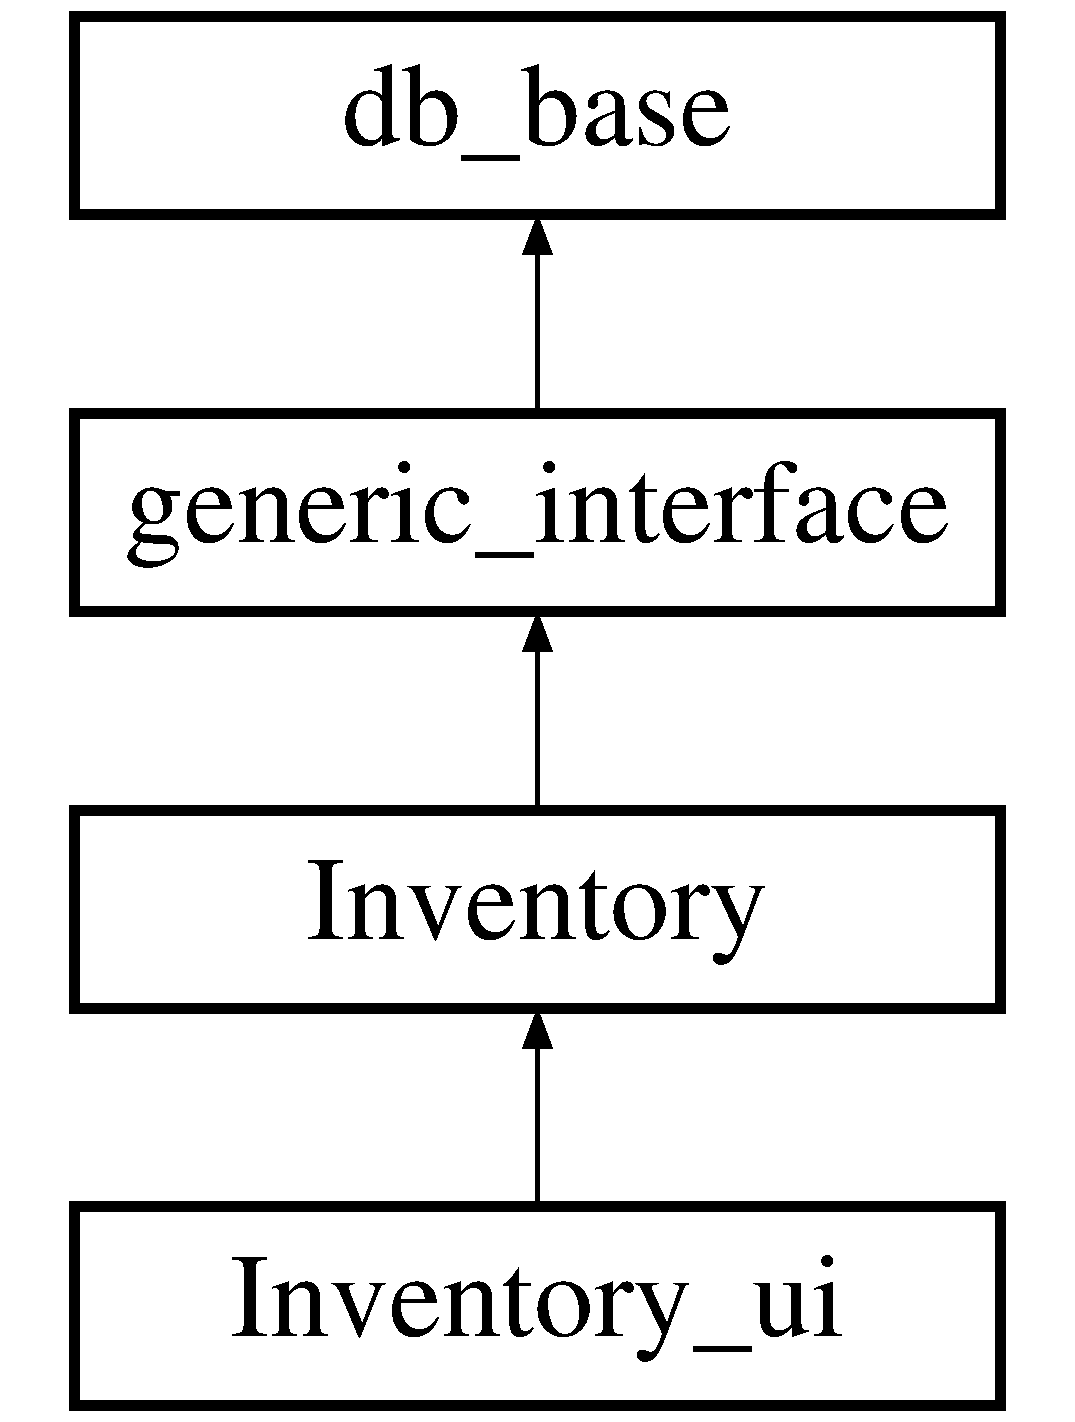
\includegraphics[height=4.000000cm]{da/d83/class_inventory__ui}
\end{center}
\end{figure}
\subsection*{Public Member Functions}
\begin{DoxyCompactItemize}
\item 
\hyperlink{class_inventory__ui_a903fc6b7eb51afa2c4f6c1392783973d}{\+\_\+\+\_\+construct} ( \$host, \$user, \$pass, \$database, \$pref\+\_\+tablename)
\item 
\hyperlink{class_inventory__ui_a107e020384575635892dd82bf07a5e46}{clearcart\+\_\+form} ()
\item 
\hyperlink{class_inventory__ui_aaa3f36bec8fb25199f697bf1983864aa}{is\+Holding\+Tank\+Set} ()
\item 
\hyperlink{class_inventory__ui_a0bdd5eda22187fd5ed67fc9b03edbbba}{handle\+P\+O\+ST} ()
\item 
\hypertarget{class_inventory__ui_ad89a4d653f5839e27c355aba1098aa8f}{}\label{class_inventory__ui_ad89a4d653f5839e27c355aba1098aa8f} 
{\bfseries submenu\+\_\+choices} ()
\item 
\hyperlink{class_inventory__ui_a5f2b542e69b9b6c8fe66d6ca513532f4}{line\+\_\+start\+\_\+focus} ()
\item 
\hyperlink{class_inventory__ui_ade75d16c1775ae3c2c40b3ac9ad6339f}{can\+\_\+process} ()
\item 
\hyperlink{class_inventory__ui_abd5a2b4048e33b9c1518db7c44115f4f}{handle\+\_\+update\+\_\+item} ()
\item 
\hyperlink{class_inventory__ui_aaa12492aec2f41782ca4467e2d0bb8c1}{handle\+\_\+delete\+\_\+item} (\$line\+\_\+no)
\item 
\hyperlink{class_inventory__ui_a37a17c8d4b2d63c774dc3404754df4f4}{get\+\_\+item\+\_\+description} ()
\item 
\hypertarget{class_inventory__ui_ab1eb2c3cdb2a43e6ff70b6ee5a0177e8}{}\label{class_inventory__ui_ab1eb2c3cdb2a43e6ff70b6ee5a0177e8} 
{\bfseries add\+\_\+item} ()
\item 
\hypertarget{class_inventory__ui_a180a927dec0a650428c79c80a55eb8a1}{}\label{class_inventory__ui_a180a927dec0a650428c79c80a55eb8a1} 
{\bfseries handle\+\_\+new\+\_\+item} ()
\item 
\hypertarget{class_inventory__ui_a7ab791c3e613331a41de68de9b5e7b63}{}\label{class_inventory__ui_a7ab791c3e613331a41de68de9b5e7b63} 
{\bfseries display\+\_\+inventory\+\_\+header} ( \$hidden\+\_\+action=\char`\"{}\char`\"{})
\item 
\hypertarget{class_inventory__ui_aa651f97c1b8cfc4a05ea091df4f0f0c8}{}\label{class_inventory__ui_aa651f97c1b8cfc4a05ea091df4f0f0c8} 
{\bfseries upc\+\_\+table} ()
\item 
\hyperlink{class_inventory__ui_af471f1ac90fef82d9f75185c7c8377f2}{module\+\_\+usage\+\_\+form} ()
\item 
\hyperlink{class_inventory__ui_a208526e58fa535e58764a7364316b4ae}{scan\+\_\+form} ()
\item 
\hypertarget{class_inventory__ui_aaf654bb6c84957067ee398ab44e3cf22}{}\label{class_inventory__ui_aaf654bb6c84957067ee398ab44e3cf22} 
{\bfseries call\+\_\+table} ( \$action, \$msg)
\item 
\hypertarget{class_inventory__ui_a86eea7fe792774c8a15ae86e07e66e2e}{}\label{class_inventory__ui_a86eea7fe792774c8a15ae86e07e66e2e} 
{\bfseries xfer\+\_\+all\+\_\+to\+\_\+location} ()
\item 
\hypertarget{class_inventory__ui_ad950a22f482e9f1a778b6771234bce42}{}\label{class_inventory__ui_ad950a22f482e9f1a778b6771234bce42} 
{\bfseries xfer\+\_\+all\+\_\+to\+\_\+holding} ()
\item 
\hyperlink{class_inventory__ui_aa78746090dbe3bcdaf4478de2efa721b}{xfer\+\_\+all\+\_\+to\+\_\+holding\+\_\+form} ()
\item 
\hyperlink{class_inventory__ui_a90577c96830f5f59f301034f4e130b2f}{xfer\+\_\+all\+\_\+to\+\_\+location\+\_\+form} ()
\item 
\hypertarget{class_inventory__ui_ad1ce51a3c48c8abb4278e93160cd1c08}{}\label{class_inventory__ui_ad1ce51a3c48c8abb4278e93160cd1c08} 
{\bfseries xferall\+\_\+form} ()
\item 
\hypertarget{class_inventory__ui_a2b914b6cf2b424e15f026edbe0e0170a}{}\label{class_inventory__ui_a2b914b6cf2b424e15f026edbe0e0170a} 
{\bfseries overunder\+\_\+form} ()
\item 
\hypertarget{class_inventory__ui_a42f3094f748f65b77fe3be03452994ac}{}\label{class_inventory__ui_a42f3094f748f65b77fe3be03452994ac} 
{\bfseries Inventory\+\_\+form} ()
\item 
\hypertarget{class_inventory__ui_a791ffee677350961cb676a08372fb479}{}\label{class_inventory__ui_a791ffee677350961cb676a08372fb479} 
{\bfseries config\+\_\+form} ()
\item 
\hypertarget{class_inventory__ui_ae2a5be945a5320013f6d973f5c9338f0}{}\label{class_inventory__ui_ae2a5be945a5320013f6d973f5c9338f0} 
{\bfseries init\+\_\+tables\+\_\+form} ()
\item 
\hypertarget{class_inventory__ui_ab88e4bea473aad102c4850f5447d0579}{}\label{class_inventory__ui_ab88e4bea473aad102c4850f5447d0579} 
{\bfseries init\+\_\+tables\+\_\+completed\+\_\+form} ()
\item 
\hypertarget{class_inventory__ui_a36f2f5f79b5aff91d0b736e92f13ff6a}{}\label{class_inventory__ui_a36f2f5f79b5aff91d0b736e92f13ff6a} 
{\bfseries process\+\_\+form} ()
\item 
\hypertarget{class_inventory__ui_a20ada151ac5c6c59298f56e00b3ebdb5}{}\label{class_inventory__ui_a20ada151ac5c6c59298f56e00b3ebdb5} 
{\bfseries display\+\_\+adjustment\+\_\+items} (\$title, \$do\+Edit=T\+R\+UE, \$show\+Stock=F\+A\+L\+SE, \$action=\char`\"{}inventory\char`\"{})
\item 
\hypertarget{class_inventory__ui_a2c9cd2fb8448bb17cbebd6394ab19522}{}\label{class_inventory__ui_a2c9cd2fb8448bb17cbebd6394ab19522} 
{\bfseries display\+\_\+inventory\+\_\+summary} (\$title, \&\$inventory, \$editable\+\_\+items=false)
\item 
\hypertarget{class_inventory__ui_a5692fdde9f762dad33c69b721365481b}{}\label{class_inventory__ui_a5692fdde9f762dad33c69b721365481b} 
{\bfseries adjustment\+\_\+edit\+\_\+item\+\_\+controls} (\$line\+\_\+no=-\/1)
\item 
\hypertarget{class_inventory__ui_a5066d159626933340a36ecf6ccbcd105}{}\label{class_inventory__ui_a5066d159626933340a36ecf6ccbcd105} 
{\bfseries adjustment\+\_\+options\+\_\+controls} ()
\item 
\hypertarget{class_inventory__ui_a494952c93f34161134321691d81cb690}{}\label{class_inventory__ui_a494952c93f34161134321691d81cb690} 
{\bfseries table\+\_\+memo\+\_\+field} ()
\item 
\hypertarget{class_inventory__ui_a0d542d348553d2eae53d09c6b50fcdc5}{}\label{class_inventory__ui_a0d542d348553d2eae53d09c6b50fcdc5} 
{\bfseries processing\+\_\+start} ()
\item 
\hypertarget{class_inventory__ui_a0b19598c5da12d8b6575839fe43ed57c}{}\label{class_inventory__ui_a0b19598c5da12d8b6575839fe43ed57c} 
{\bfseries processing\+\_\+end} ()
\item 
\hypertarget{class_inventory__ui_a3f96b768221aab8a1676c18cc9acc06c}{}\label{class_inventory__ui_a3f96b768221aab8a1676c18cc9acc06c} 
{\bfseries confirm\+\_\+dialog} (\$submit, \$msg)
\item 
\hypertarget{class_inventory__ui_ad48e9be2b4334c75b632a1fc3280a462}{}\label{class_inventory__ui_ad48e9be2b4334c75b632a1fc3280a462} 
{\bfseries page\+\_\+processing} (\$msg=false)
\item 
\hypertarget{class_inventory__ui_a8348636c222a752d1eb99e368eadd142}{}\label{class_inventory__ui_a8348636c222a752d1eb99e368eadd142} 
{\bfseries page\+\_\+modified} (\$status=true)
\end{DoxyCompactItemize}
\subsection*{Additional Inherited Members}


\subsection{Detailed Description}
Class \hyperlink{class_inventory}{Inventory} is the routines for doing a stock taking.

Class \hyperlink{class_inventory}{Inventory} is the routines for doing a stock taking. It also allows you to do inventory transfers of A\+LL inventory without having to count those items at both locations. A\+S\+S\+U\+M\+P\+T\+I\+ON is that you will do an appropriate inventory count later. 

\subsection{Constructor \& Destructor Documentation}
\hypertarget{class_inventory__ui_a903fc6b7eb51afa2c4f6c1392783973d}{}\label{class_inventory__ui_a903fc6b7eb51afa2c4f6c1392783973d} 
\index{Inventory\+\_\+ui@{Inventory\+\_\+ui}!\+\_\+\+\_\+construct@{\+\_\+\+\_\+construct}}
\index{\+\_\+\+\_\+construct@{\+\_\+\+\_\+construct}!Inventory\+\_\+ui@{Inventory\+\_\+ui}}
\subsubsection{\texorpdfstring{\+\_\+\+\_\+construct()}{\_\_construct()}}
{\footnotesize\ttfamily Inventory\+\_\+ui\+::\+\_\+\+\_\+construct (\begin{DoxyParamCaption}\item[{}]{\$host,  }\item[{}]{\$user,  }\item[{}]{\$pass,  }\item[{}]{\$database,  }\item[{}]{\$pref\+\_\+tablename }\end{DoxyParamCaption})}

Constructor

The params for this constructor are not needed for this particular function; They are needed for compatibility to \hyperlink{classgeneric__interface}{generic\+\_\+interface} which this class extends so that we don\textquotesingle{}t break the parent constructor.

Generic\+\_\+interface gives us the routines that allow us to set actions and the forms/routines that we are supposed to then call without having to write a bunch of if/then/else statements. (see \$this-\/$>$tabs). It also gives us the generic C\+O\+N\+F\+IG V\+A\+R\+I\+A\+B\+L\+ES (see \$this-\/$>$config\+\_\+values) which are then presented on the configuration tab, and stored in the modules prefs table.


\begin{DoxyParams}[2]{Parameters}
\mbox{\tt in}  & string & {\em \$host} & server name for connection to the database \\
\hline
\mbox{\tt in}  & string & {\em \$user} & username for connecting to the database \\
\hline
\mbox{\tt in}  & string & {\em \$pass} & password for connecting to the database \\
\hline
\mbox{\tt in}  & string & {\em \$database} & database name \\
\hline
\mbox{\tt in}  & string & {\em \$pref\+\_\+tablename} & The name of the table storing the preferences (config) of this class \\
\hline
\end{DoxyParams}


\subsection{Member Function Documentation}
\hypertarget{class_inventory__ui_ade75d16c1775ae3c2c40b3ac9ad6339f}{}\label{class_inventory__ui_ade75d16c1775ae3c2c40b3ac9ad6339f} 
\index{Inventory\+\_\+ui@{Inventory\+\_\+ui}!can\+\_\+process@{can\+\_\+process}}
\index{can\+\_\+process@{can\+\_\+process}!Inventory\+\_\+ui@{Inventory\+\_\+ui}}
\subsubsection{\texorpdfstring{can\+\_\+process()}{can\_process()}}
{\footnotesize\ttfamily Inventory\+\_\+ui\+::can\+\_\+process (\begin{DoxyParamCaption}{ }\end{DoxyParamCaption})}

Can we process the data of the cart?

\begin{DoxySeeAlso}{See also}
(\hyperlink{class_inventory}{Inventory})\hyperlink{class_inventory__ui_ade75d16c1775ae3c2c40b3ac9ad6339f}{can\+\_\+process()} 
\end{DoxySeeAlso}
\begin{DoxyReturn}{Returns}
bool Yes we can or Not 
\end{DoxyReturn}
\hypertarget{class_inventory__ui_a107e020384575635892dd82bf07a5e46}{}\label{class_inventory__ui_a107e020384575635892dd82bf07a5e46} 
\index{Inventory\+\_\+ui@{Inventory\+\_\+ui}!clearcart\+\_\+form@{clearcart\+\_\+form}}
\index{clearcart\+\_\+form@{clearcart\+\_\+form}!Inventory\+\_\+ui@{Inventory\+\_\+ui}}
\subsubsection{\texorpdfstring{clearcart\+\_\+form()}{clearcart\_form()}}
{\footnotesize\ttfamily Inventory\+\_\+ui\+::clearcart\+\_\+form (\begin{DoxyParamCaption}{ }\end{DoxyParamCaption})}

Clear the cart of all items \hypertarget{class_inventory__ui_a37a17c8d4b2d63c774dc3404754df4f4}{}\label{class_inventory__ui_a37a17c8d4b2d63c774dc3404754df4f4} 
\index{Inventory\+\_\+ui@{Inventory\+\_\+ui}!get\+\_\+item\+\_\+description@{get\+\_\+item\+\_\+description}}
\index{get\+\_\+item\+\_\+description@{get\+\_\+item\+\_\+description}!Inventory\+\_\+ui@{Inventory\+\_\+ui}}
\subsubsection{\texorpdfstring{get\+\_\+item\+\_\+description()}{get\_item\_description()}}
{\footnotesize\ttfamily Inventory\+\_\+ui\+::get\+\_\+item\+\_\+description (\begin{DoxyParamCaption}{ }\end{DoxyParamCaption})}

Get the description from stock\+\_\+master for the item \begin{DoxyWarning}{Warning}
expects stock\+\_\+id to be set 
\end{DoxyWarning}
\hypertarget{class_inventory__ui_aaa12492aec2f41782ca4467e2d0bb8c1}{}\label{class_inventory__ui_aaa12492aec2f41782ca4467e2d0bb8c1} 
\index{Inventory\+\_\+ui@{Inventory\+\_\+ui}!handle\+\_\+delete\+\_\+item@{handle\+\_\+delete\+\_\+item}}
\index{handle\+\_\+delete\+\_\+item@{handle\+\_\+delete\+\_\+item}!Inventory\+\_\+ui@{Inventory\+\_\+ui}}
\subsubsection{\texorpdfstring{handle\+\_\+delete\+\_\+item()}{handle\_delete\_item()}}
{\footnotesize\ttfamily Inventory\+\_\+ui\+::handle\+\_\+delete\+\_\+item (\begin{DoxyParamCaption}\item[{}]{\$line\+\_\+no }\end{DoxyParamCaption})}

Handle the deleting from the cart of an item \hypertarget{class_inventory__ui_abd5a2b4048e33b9c1518db7c44115f4f}{}\label{class_inventory__ui_abd5a2b4048e33b9c1518db7c44115f4f} 
\index{Inventory\+\_\+ui@{Inventory\+\_\+ui}!handle\+\_\+update\+\_\+item@{handle\+\_\+update\+\_\+item}}
\index{handle\+\_\+update\+\_\+item@{handle\+\_\+update\+\_\+item}!Inventory\+\_\+ui@{Inventory\+\_\+ui}}
\subsubsection{\texorpdfstring{handle\+\_\+update\+\_\+item()}{handle\_update\_item()}}
{\footnotesize\ttfamily Inventory\+\_\+ui\+::handle\+\_\+update\+\_\+item (\begin{DoxyParamCaption}{ }\end{DoxyParamCaption})}

Handle the updating of the count of a stock\+\_\+id \hypertarget{class_inventory__ui_a0bdd5eda22187fd5ed67fc9b03edbbba}{}\label{class_inventory__ui_a0bdd5eda22187fd5ed67fc9b03edbbba} 
\index{Inventory\+\_\+ui@{Inventory\+\_\+ui}!handle\+P\+O\+ST@{handle\+P\+O\+ST}}
\index{handle\+P\+O\+ST@{handle\+P\+O\+ST}!Inventory\+\_\+ui@{Inventory\+\_\+ui}}
\subsubsection{\texorpdfstring{handle\+P\+O\+S\+T()}{handlePOST()}}
{\footnotesize\ttfamily Inventory\+\_\+ui\+::handle\+P\+O\+ST (\begin{DoxyParamCaption}{ }\end{DoxyParamCaption})}

Handle the variables we are expecting to be set somewhere in this class on a form

\begin{DoxyWarning}{Warning}
calls Ajax calls in the browser 
\end{DoxyWarning}
\hypertarget{class_inventory__ui_aaa3f36bec8fb25199f697bf1983864aa}{}\label{class_inventory__ui_aaa3f36bec8fb25199f697bf1983864aa} 
\index{Inventory\+\_\+ui@{Inventory\+\_\+ui}!is\+Holding\+Tank\+Set@{is\+Holding\+Tank\+Set}}
\index{is\+Holding\+Tank\+Set@{is\+Holding\+Tank\+Set}!Inventory\+\_\+ui@{Inventory\+\_\+ui}}
\subsubsection{\texorpdfstring{is\+Holding\+Tank\+Set()}{isHoldingTankSet()}}
{\footnotesize\ttfamily Inventory\+\_\+ui\+::is\+Holding\+Tank\+Set (\begin{DoxyParamCaption}{ }\end{DoxyParamCaption})}

Check that the holding tank variable has been set. Needed for transfers to work correctly.

\begin{DoxyReturn}{Returns}
Bool set or not 
\end{DoxyReturn}
\hypertarget{class_inventory__ui_a5f2b542e69b9b6c8fe66d6ca513532f4}{}\label{class_inventory__ui_a5f2b542e69b9b6c8fe66d6ca513532f4} 
\index{Inventory\+\_\+ui@{Inventory\+\_\+ui}!line\+\_\+start\+\_\+focus@{line\+\_\+start\+\_\+focus}}
\index{line\+\_\+start\+\_\+focus@{line\+\_\+start\+\_\+focus}!Inventory\+\_\+ui@{Inventory\+\_\+ui}}
\subsubsection{\texorpdfstring{line\+\_\+start\+\_\+focus()}{line\_start\_focus()}}
{\footnotesize\ttfamily Inventory\+\_\+ui\+::line\+\_\+start\+\_\+focus (\begin{DoxyParamCaption}{ }\end{DoxyParamCaption})}

Set the focus on the cart\textquotesingle{}s displayed table and put the cursor into the U\+PC edit box

\begin{DoxyReturn}{Returns}
N\+O\+NE 
\end{DoxyReturn}
\hypertarget{class_inventory__ui_af471f1ac90fef82d9f75185c7c8377f2}{}\label{class_inventory__ui_af471f1ac90fef82d9f75185c7c8377f2} 
\index{Inventory\+\_\+ui@{Inventory\+\_\+ui}!module\+\_\+usage\+\_\+form@{module\+\_\+usage\+\_\+form}}
\index{module\+\_\+usage\+\_\+form@{module\+\_\+usage\+\_\+form}!Inventory\+\_\+ui@{Inventory\+\_\+ui}}
\subsubsection{\texorpdfstring{module\+\_\+usage\+\_\+form()}{module\_usage\_form()}}
{\footnotesize\ttfamily Inventory\+\_\+ui\+::module\+\_\+usage\+\_\+form (\begin{DoxyParamCaption}{ }\end{DoxyParamCaption})}

Form to show how to use the module.


\begin{DoxyParams}{Parameters}
{\em N\+O\+NE} & \\
\hline
\end{DoxyParams}
\begin{DoxyReturn}{Returns}
N\+O\+NE 
\end{DoxyReturn}
\hypertarget{class_inventory__ui_a208526e58fa535e58764a7364316b4ae}{}\label{class_inventory__ui_a208526e58fa535e58764a7364316b4ae} 
\index{Inventory\+\_\+ui@{Inventory\+\_\+ui}!scan\+\_\+form@{scan\+\_\+form}}
\index{scan\+\_\+form@{scan\+\_\+form}!Inventory\+\_\+ui@{Inventory\+\_\+ui}}
\subsubsection{\texorpdfstring{scan\+\_\+form()}{scan\_form()}}
{\footnotesize\ttfamily Inventory\+\_\+ui\+::scan\+\_\+form (\begin{DoxyParamCaption}{ }\end{DoxyParamCaption})}

Scan a U\+PC and if a product add to the count of items in the cart.


\begin{DoxyParams}{Parameters}
{\em N\+O\+NE} & \\
\hline
\end{DoxyParams}
\begin{DoxyReturn}{Returns}
N\+O\+NE 
\end{DoxyReturn}
\hypertarget{class_inventory__ui_aa78746090dbe3bcdaf4478de2efa721b}{}\label{class_inventory__ui_aa78746090dbe3bcdaf4478de2efa721b} 
\index{Inventory\+\_\+ui@{Inventory\+\_\+ui}!xfer\+\_\+all\+\_\+to\+\_\+holding\+\_\+form@{xfer\+\_\+all\+\_\+to\+\_\+holding\+\_\+form}}
\index{xfer\+\_\+all\+\_\+to\+\_\+holding\+\_\+form@{xfer\+\_\+all\+\_\+to\+\_\+holding\+\_\+form}!Inventory\+\_\+ui@{Inventory\+\_\+ui}}
\subsubsection{\texorpdfstring{xfer\+\_\+all\+\_\+to\+\_\+holding\+\_\+form()}{xfer\_all\_to\_holding\_form()}}
{\footnotesize\ttfamily Inventory\+\_\+ui\+::xfer\+\_\+all\+\_\+to\+\_\+holding\+\_\+form (\begin{DoxyParamCaption}{ }\end{DoxyParamCaption})}

xfer\+\_\+all\+\_\+to\+\_\+holding\+\_\+form displays a button to initiate the transfer

This function displays the form with a button to initiate a transfer of A\+LL inventory at a location to the H\+O\+L\+D\+I\+NG tank. It zero\textquotesingle{}s the inventory count for any items that have more than 0 items showing as on hand. \hypertarget{class_inventory__ui_a90577c96830f5f59f301034f4e130b2f}{}\label{class_inventory__ui_a90577c96830f5f59f301034f4e130b2f} 
\index{Inventory\+\_\+ui@{Inventory\+\_\+ui}!xfer\+\_\+all\+\_\+to\+\_\+location\+\_\+form@{xfer\+\_\+all\+\_\+to\+\_\+location\+\_\+form}}
\index{xfer\+\_\+all\+\_\+to\+\_\+location\+\_\+form@{xfer\+\_\+all\+\_\+to\+\_\+location\+\_\+form}!Inventory\+\_\+ui@{Inventory\+\_\+ui}}
\subsubsection{\texorpdfstring{xfer\+\_\+all\+\_\+to\+\_\+location\+\_\+form()}{xfer\_all\_to\_location\_form()}}
{\footnotesize\ttfamily Inventory\+\_\+ui\+::xfer\+\_\+all\+\_\+to\+\_\+location\+\_\+form (\begin{DoxyParamCaption}{ }\end{DoxyParamCaption})}

xfer\+\_\+all\+\_\+to\+\_\+location\+\_\+form displays a button to initiate the transfer

This function displays the form with a button to initiate a transfer of A\+LL inventory from one location to another. It zero\textquotesingle{}s the inventory count for any items that have more than 0 items showing as on hand at the F\+R\+OM location and using FA routines transfers that count to the TO location. 

The documentation for this class was generated from the following file\+:\begin{DoxyCompactItemize}
\item 
class.\+Inventory\+\_\+ui.\+php\end{DoxyCompactItemize}

\hypertarget{classitem}{}\section{item Class Reference}
\label{classitem}\index{item@{item}}
\subsection*{Public Member Functions}
\begin{DoxyCompactItemize}
\item 
\hyperlink{classitem_a6034ca2afb124263ba90707959afaf41}{\+\_\+\+\_\+construct} ( \$stock\+\_\+id, \$location=-\/1)
\item 
\hypertarget{classitem_ac76cffc0c8c70c5e5aaeda74e35a55f8}{}\label{classitem_ac76cffc0c8c70c5e5aaeda74e35a55f8} 
{\bfseries update\+\_\+counted} ( \$count)
\item 
\hypertarget{classitem_aa3b7b9f2808a49c87af5043f38dd59d3}{}\label{classitem_aa3b7b9f2808a49c87af5043f38dd59d3} 
{\bfseries increase\+\_\+count} ( \$count)
\item 
\hypertarget{classitem_a210605b6202b2951189d6848fcd54b6e}{}\label{classitem_a210605b6202b2951189d6848fcd54b6e} 
{\bfseries is\+\_\+me} ( \$stock\+\_\+id)
\item 
\hypertarget{classitem_ac8ddae8b84bb5d8c044b0779e1843542}{}\label{classitem_ac8ddae8b84bb5d8c044b0779e1843542} 
{\bfseries get\+\_\+stock\+\_\+id} ( \$item\+\_\+code)
\item 
\hyperlink{classitem_a17a922f5ec3b2241675aea5ef0fdc8d5}{is\+Stockid} ( \$stock\+\_\+id)
\item 
\hyperlink{classitem_a9d1f895627df632f2134f0161d5da726}{is\+Item\+Code} ( \$item\+\_\+code)
\item 
\hyperlink{classitem_ac1e7020aea1578a37ba70dd37ba5ca13}{get\+\_\+item\+\_\+description} ()
\item 
\hyperlink{classitem_aa76507a7473d77d4f2472616abcb664f}{get\+\_\+item\+\_\+qoh\+\_\+location} ( \$stock\+\_\+id)
\end{DoxyCompactItemize}
\subsection*{Public Attributes}
\begin{DoxyCompactItemize}
\item 
\hypertarget{classitem_a960d2ea48d7f3b60b7fe360e10b331f7}{}\label{classitem_a960d2ea48d7f3b60b7fe360e10b331f7} 
\hyperlink{classitem_a960d2ea48d7f3b60b7fe360e10b331f7}{\$location}
\begin{DoxyCompactList}\small\item\em \hyperlink{class_inventory}{Inventory} location. \end{DoxyCompactList}\item 
\hypertarget{classitem_a1d115888a094a2d8b1af138cb872dadd}{}\label{classitem_a1d115888a094a2d8b1af138cb872dadd} 
{\bfseries \$barcode}
\item 
\hypertarget{classitem_a06cded759cb0ed22235de6288a6d56be}{}\label{classitem_a06cded759cb0ed22235de6288a6d56be} 
{\bfseries \$title}
\item 
\hypertarget{classitem_a3bd53b1d94f98aaea6065fd652d21962}{}\label{classitem_a3bd53b1d94f98aaea6065fd652d21962} 
{\bfseries \$stock\+\_\+id}
\item 
\hypertarget{classitem_a3a05562f1a44a3afbde5af0382503e8e}{}\label{classitem_a3a05562f1a44a3afbde5af0382503e8e} 
{\bfseries \$description}
\item 
\hypertarget{classitem_aa8fccc6e8adc31bc3f93609244f8b6a8}{}\label{classitem_aa8fccc6e8adc31bc3f93609244f8b6a8} 
{\bfseries \$debug}
\item 
\hypertarget{classitem_a4bc44758eac5607db2febc8fb03a47aa}{}\label{classitem_a4bc44758eac5607db2febc8fb03a47aa} 
\hyperlink{classitem_a4bc44758eac5607db2febc8fb03a47aa}{\$qoh}
\begin{DoxyCompactList}\small\item\em How many FA thinks we have at this location. \end{DoxyCompactList}\item 
\hypertarget{classitem_aab048fbbe2ff803cf2367fa465be0f3a}{}\label{classitem_aab048fbbe2ff803cf2367fa465be0f3a} 
\hyperlink{classitem_aab048fbbe2ff803cf2367fa465be0f3a}{\$counted}
\begin{DoxyCompactList}\small\item\em How many we have counted at this location. \end{DoxyCompactList}\end{DoxyCompactItemize}


\subsection{Detailed Description}
Class \hyperlink{class_inventory}{Inventory} is the routines for doing a stock taking.

Class \hyperlink{class_inventory}{Inventory} is the routines for doing a stock taking. It also allows you to do inventory transfers of A\+LL inventory without having to count those items at both locations. A\+S\+S\+U\+M\+P\+T\+I\+ON is that you will do an appropriate inventory count later. 

\subsection{Constructor \& Destructor Documentation}
\hypertarget{classitem_a6034ca2afb124263ba90707959afaf41}{}\label{classitem_a6034ca2afb124263ba90707959afaf41} 
\index{item@{item}!\+\_\+\+\_\+construct@{\+\_\+\+\_\+construct}}
\index{\+\_\+\+\_\+construct@{\+\_\+\+\_\+construct}!item@{item}}
\subsubsection{\texorpdfstring{\+\_\+\+\_\+construct()}{\_\_construct()}}
{\footnotesize\ttfamily item\+::\+\_\+\+\_\+construct (\begin{DoxyParamCaption}\item[{}]{\$stock\+\_\+id,  }\item[{}]{\$location = {\ttfamily -\/1} }\end{DoxyParamCaption})}

Constructor


\begin{DoxyParams}{Parameters}
{\em string} & stock\+\_\+id \\
\hline
{\em string} & location identifier \\
\hline
{\em string} & date \\
\hline
\end{DoxyParams}
\begin{DoxyReturn}{Returns}
null 
\end{DoxyReturn}


\subsection{Member Function Documentation}
\hypertarget{classitem_ac1e7020aea1578a37ba70dd37ba5ca13}{}\label{classitem_ac1e7020aea1578a37ba70dd37ba5ca13} 
\index{item@{item}!get\+\_\+item\+\_\+description@{get\+\_\+item\+\_\+description}}
\index{get\+\_\+item\+\_\+description@{get\+\_\+item\+\_\+description}!item@{item}}
\subsubsection{\texorpdfstring{get\+\_\+item\+\_\+description()}{get\_item\_description()}}
{\footnotesize\ttfamily item\+::get\+\_\+item\+\_\+description (\begin{DoxyParamCaption}{ }\end{DoxyParamCaption})}

retrieve item\textquotesingle{}s description. Depends on stock\+\_\+id being set

\begin{DoxyReturn}{Returns}
bool whether we retrieved or not. 
\end{DoxyReturn}
\hypertarget{classitem_aa76507a7473d77d4f2472616abcb664f}{}\label{classitem_aa76507a7473d77d4f2472616abcb664f} 
\index{item@{item}!get\+\_\+item\+\_\+qoh\+\_\+location@{get\+\_\+item\+\_\+qoh\+\_\+location}}
\index{get\+\_\+item\+\_\+qoh\+\_\+location@{get\+\_\+item\+\_\+qoh\+\_\+location}!item@{item}}
\subsubsection{\texorpdfstring{get\+\_\+item\+\_\+qoh\+\_\+location()}{get\_item\_qoh\_location()}}
{\footnotesize\ttfamily item\+::get\+\_\+item\+\_\+qoh\+\_\+location (\begin{DoxyParamCaption}\item[{}]{\$stock\+\_\+id }\end{DoxyParamCaption})}

retrieve item\textquotesingle{}s Q\+OH on a date. Depends on stock\+\_\+id, location, document\+\_\+date being set

\begin{DoxyReturn}{Returns}
bool whether we retrieved or not. 
\end{DoxyReturn}
\hypertarget{classitem_a9d1f895627df632f2134f0161d5da726}{}\label{classitem_a9d1f895627df632f2134f0161d5da726} 
\index{item@{item}!is\+Item\+Code@{is\+Item\+Code}}
\index{is\+Item\+Code@{is\+Item\+Code}!item@{item}}
\subsubsection{\texorpdfstring{is\+Item\+Code()}{isItemCode()}}
{\footnotesize\ttfamily item\+::is\+Item\+Code (\begin{DoxyParamCaption}\item[{}]{\$item\+\_\+code }\end{DoxyParamCaption})}

check for a foreign/part code. Sets stock\+\_\+id if found.


\begin{DoxyParams}{Parameters}
{\em string} & stock\+\_\+id/item\+\_\+code \\
\hline
\end{DoxyParams}
\begin{DoxyReturn}{Returns}
bool whether item is in item\+\_\+codes A\+ND stock\+\_\+id$<$$>$item\+\_\+code 
\end{DoxyReturn}
\hypertarget{classitem_a17a922f5ec3b2241675aea5ef0fdc8d5}{}\label{classitem_a17a922f5ec3b2241675aea5ef0fdc8d5} 
\index{item@{item}!is\+Stockid@{is\+Stockid}}
\index{is\+Stockid@{is\+Stockid}!item@{item}}
\subsubsection{\texorpdfstring{is\+Stockid()}{isStockid()}}
{\footnotesize\ttfamily item\+::is\+Stockid (\begin{DoxyParamCaption}\item[{}]{\$stock\+\_\+id }\end{DoxyParamCaption})}

Is the item in the ?stock\+\_\+master? databas


\begin{DoxyParams}{Parameters}
{\em string} & the stock\+\_\+id to check \\
\hline
\end{DoxyParams}
\begin{DoxyReturn}{Returns}
bool Is the item in the ?stock\+\_\+master? database 
\end{DoxyReturn}


The documentation for this class was generated from the following file\+:\begin{DoxyCompactItemize}
\item 
class.\+item.\+php\end{DoxyCompactItemize}

%--- End generated contents ---

% Index
\backmatter
\newpage
\phantomsection
\clearemptydoublepage
\addcontentsline{toc}{chapter}{Index}
\printindex

\end{document}
